\documentclass[11pt,a4paper]{report}

% --- Tipografía y Configuración de Página ---
\usepackage[utf8]{inputenc}
\usepackage[T1]{fontenc}
\usepackage[spanish,es-nodecimaldot]{babel}
\usepackage{helvet}
\renewcommand{\familydefault}{\sfdefault}
\usepackage[margin=2.4cm,top=2.6cm,bottom=2.6cm,headheight=16pt]{geometry}
\usepackage{graphicx}
\usepackage{xcolor}
\usepackage{titlesec}
\usepackage{fancyhdr}
\usepackage{booktabs}
\usepackage{tabularx}
\usepackage{array}
\usepackage{enumitem}
\usepackage{tcolorbox}
\tcbuselibrary{skins,breakable}
\usepackage{microtype}
\usepackage{float}
\usepackage{amsmath,amssymb}
\usepackage[
    colorlinks=true,
    linkcolor=MaizPrimary,
    urlcolor=MaizLightGreen,
    citecolor=MaizDarkGreen,
    pdfauthor={Equipo Técnico de Doctor Maíz},
    pdftitle={Doctor Maíz - Manual Práctico de Usuario y Guía de Campo},
    pdfsubject={Manual de Usuario Completo para la App Móvil Doctor Maíz},
    pdfkeywords={Maíz, Agricultura de Precisión, Diagnóstico Foliar, Android, Guía de Campo}
]{hyperref}

% --- Paleta de Color Institucional ---
\definecolor{MaizDarkGreen}{HTML}{1B4332}
\definecolor{MaizPrimary}{HTML}{2D6A4F}
\definecolor{MaizLightGreen}{HTML}{40916C}
\definecolor{MaizMint}{HTML}{52B788}
\definecolor{MaizPaleGreen}{HTML}{E8F5E9}
\definecolor{MaizGold}{HTML}{D4A373}
\definecolor{MaizRed}{HTML}{BA1A1A}
\definecolor{MaizRedBg}{HTML}{FFEBEE}
\definecolor{MaizDark}{HTML}{1A202C}
\definecolor{MaizGray}{HTML}{4A5568}
\definecolor{MaizLightGray}{HTML}{F8FAFC}
\definecolor{MaizBorder}{HTML}{E2E8F0}

% --- Cajas de Campo y Recomendaciones Prácticas ---
\newtcolorbox{pasoapaso}[1][]{
    enhanced,
    breakable,
    colback=white,
    colframe=MaizPrimary,
    coltitle=white,
    fonttitle=\bfseries\sffamily,
    title={Paso a Paso en Campo},
    attach boxed title to top left={yshift=-2mm,xshift=5mm},
    boxed title style={sharp corners, rounded corners=southeast, colback=MaizPrimary},
    arc=2.5mm,
    boxrule=1.2pt,
    left=4mm, right=4mm, top=4mm, bottom=4mm,
    #1
}

\newtcolorbox{agronote}[1][]{
    enhanced,
    breakable,
    colback=MaizPaleGreen,
    colframe=MaizPrimary,
    coltitle=white,
    fonttitle=\bfseries\sffamily,
    title={Criterio Agronómico},
    attach boxed title to top left={yshift=-2mm,xshift=5mm},
    boxed title style={sharp corners, rounded corners=southeast, colback=MaizPrimary},
    arc=2.5mm,
    boxrule=1.2pt,
    left=4mm, right=4mm, top=4mm, bottom=4mm,
    #1
}

\newtcolorbox{agroalert}[1][]{
    enhanced,
    breakable,
    colback=MaizRedBg,
    colframe=MaizRed,
    coltitle=white,
    fonttitle=\bfseries\sffamily,
    title={Atención en el Lote},
    attach boxed title to top left={yshift=-2mm,xshift=5mm},
    boxed title style={sharp corners, rounded corners=southeast, colback=MaizRed},
    arc=2.5mm,
    boxrule=1.2pt,
    left=4mm, right=4mm, top=4mm, bottom=4mm,
    #1
}

\newtcolorbox{campotip}[1][]{
    enhanced,
    breakable,
    colback=MaizLightGray,
    colframe=MaizGold,
    coltitle=MaizDark,
    fonttitle=\bfseries\sffamily,
    title={Recomendación Práctica},
    attach boxed title to top left={yshift=-2mm,xshift=5mm},
    boxed title style={sharp corners, rounded corners=southeast, colback=MaizGold},
    arc=2.5mm,
    boxrule=1.2pt,
    left=4mm, right=4mm, top=4mm, bottom=4mm,
    #1
}

% --- Estilo de Títulos de Capítulos y Secciones ---
\titleformat{\chapter}[display]
{\normalfont\sffamily\huge\bfseries\color{MaizDarkGreen}}
{\filleft\Huge\color{MaizMint}\chaptertitlename\ \thechapter}
{0.5ex}
{\titlerule[2pt]\vspace{1ex}\filright}
[\vspace{1ex}\titlerule]

\titleformat{\section}
{\normalfont\sffamily\Large\bfseries\color{MaizPrimary}}
{\thesection}{1em}{}[{\color{MaizMint}\titlerule[1pt]}]

\titleformat{\subsection}
{\normalfont\sffamily\large\bfseries\color{MaizDarkGreen}}
{\thesubsection}{1em}{}

% --- Encabezados y Pie de Página ---
\pagestyle{fancy}
\fancyhf{}
\fancyhead[L]{\small\color{MaizGray}\textsf{Doctor Maíz --- Manual de Usuario}}
\fancyhead[R]{\small\color{MaizPrimary}\textsf{\leftmark}}
\fancyfoot[C]{\thepage}
\fancyfoot[R]{\small\color{MaizGray}\textsf{v1.0.0 Nativo}}
\renewcommand{\headrulewidth}{0.5pt}
\renewcommand{\footrulewidth}{0.3pt}
\renewcommand{\chaptermark}[1]{\markboth{#1}{}}

% -------------------------------------------------------------
% COMIENZO DEL DOCUMENTO
% -------------------------------------------------------------
\begin{document}
\pagenumbering{roman}

% --- PORTADA ---
\begin{titlepage}
    \pagecolor{MaizDarkGreen}
    \color{white}
    \begin{center}
        \vspace*{1.2cm}
        
        
\includegraphics[width=3.4cm]{img/app_icon.png}
        
        \vspace{1.0cm}
        
        {\Huge \textbf{\textsf{DOCTOR MAÍZ}}}\\[0.3cm]
        {\Large \textsf{Manual Práctico de Usuario y Operación en Campo}}\\[0.2cm]
        {\large \textsf{Diagnóstico en el Surco, Georreferenciación y Manejo de Cultivo}}
        
        \vspace{1.2cm}
        
        \noindent\makebox[\linewidth]{\color{MaizMint}\rule{0.85\linewidth}{2pt}}
        
        \vspace{1.2cm}
        
        {\LARGE \textbf{\textsf{GUÍA COMPLETA PASO A PASO}}}\\[0.4cm]
        {\normalsize \textsf{Instalación, cuentas, escaneo con IA local, mapas de lote y buenas prácticas}}
        
        \vfill
        
        \begin{tcolorbox}[colback=white!10!MaizDarkGreen,colframe=MaizMint,arc=3mm,width=0.92\linewidth]
            \centering\small
            \textbf{Aplicación Móvil:} Doctor Maíz v1.0.0 para Android\\
            \textbf{Dispositivo de Referencia:} Google Pixel 4 / Android 7.0+\\
            \textbf{Modalidad de Operación:} 100\% Fuera de Línea (Edge AI)\\
            \textbf{Última Actualización:} Septiembre 2026
        \end{tcolorbox}
        
        \vspace{0.6cm}
    \end{center}
\end{titlepage}
\nopagecolor

% --- PÁGINA EDITORIAL Y ACLARACIÓN DE CAMPO ---
\thispagestyle{empty}
\vspace*{1.5cm}
\noindent\textbf{Doctor Maíz: Manual Práctico de Usuario y Operación en Campo}\\
\noindent\textcopyright\ 2026 Proyecto Doctor Maíz. Desarrollado para productores, técnicos y extensionistas agrícolas.\\
\noindent Todos los derechos reservados.

\vspace{0.8cm}
\noindent\textbf{Sobre esta guía:}\\
\small
Este manual explica cómo usar la aplicación desde el momento en que recibes el archivo de instalación en tu teléfono hasta que realizas recorridos completos de diagnóstico en tu parcela. El objetivo es que cualquier persona, sin importar su experiencia previa con tecnología, pueda identificar rápidamente qué problema tiene su maíz y qué hacer para proteger su cosecha sin gastar de más en agroquímicos innecesarios.

\vspace{0.6cm}
\noindent\textbf{Aviso sobre los diagnósticos:}\\
Doctor Maíz es un asistente de apoyo basado en visión artificial que analiza los patrones visuales de las hojas. Te ayuda a saber qué patógeno o deficiencia nutricional está presente y te brinda descripciones para que compares el nivel de daño. La aplicación no sustituye las visitas de un profesional agrónomo ni las pruebas de laboratorio de suelo o tejido. Frente a una duda grave o síntomas atípicos en tu zona, consulta con el extensionista o la agencia agrícola de tu comunidad.

\vfill
\noindent\textbf{Módulos documentados:} Instalación de APK, Permisos del sistema, Registro e Inicio de Sesión, Modo Invitado sin conexión, Perfil del productor, Sincronización en la nube, Pantalla de Inicio y Clima, Cámara con Retícula Foliar, Guía de Severidad en 3 Niveles, Catálogo de 9 Patologías, Mapa Satelital de Lotes, Historial de Muestreos y Contribución al Dataset Nacional.

\newpage

% --- ÍNDICE GENERAL ---
\tableofcontents
\newpage

\pagenumbering{arabic}
\setcounter{page}{1}

% -------------------------------------------------------------
% CAPÍTULO 1: INSTALACIÓN Y CONFIGURACIÓN INICIAL
% -------------------------------------------------------------
\chapter{Instalación y Configuración Inicial}

\section{Requisitos del Teléfono}
Doctor Maíz fue construida pensando en la realidad del campo: caminos de tierra, polvo, calor y muchas zonas donde la señal de celular es débil o nula. Por eso, todo el procesamiento pesado de imágenes ocurre dentro de tu propio teléfono mediante un modelo de inteligencia artificial optimizado.

Para que la aplicación funcione con fluidez, tu teléfono debe contar con:
\begin{itemize}
    \item \textbf{Sistema Operativo:} Android 7.0 (Nougat) o cualquier versión superior (probado y optimizado en teléfonos como el Google Pixel 4 y similares).
    \item \textbf{Cámara con Enfoque Automático:} Lente trasera de al menos 8 megapíxeles (recomendable 12 MP o más) para distinguir con nitidez lesiones pequeñas o pústulas de roya.
    \item \textbf{Ubicación (GPS):} Sensor GPS activo para ubicar cada muestra dentro de tu lote.
    \item \textbf{Memoria y Espacio:} Mínimo 2 GB de memoria RAM y unos 150 MB libres de almacenamiento interno para el modelo neuronal y el catálogo de imágenes.
\end{itemize}

\section{Instalación del Archivo APK}
Si recibiste la aplicación mediante un enlace de descarga, memoria USB, Bluetooth o a través de WhatsApp mediante el archivo \texttt{DoctorMaiz-v1.0.0.apk}, sigue estos pasos:

\begin{pasoapaso}
\begin{enumerate}
    \item \textbf{Abrir el archivo descargado:} Ve a la carpeta \textit{Descargas} de tu teléfono y toca el archivo \texttt{DoctorMaiz-v1.0.0.apk}.
    \item \textbf{Permitir instalación de fuentes desconocidas:} Si Android te muestra una advertencia de seguridad indicando que tu navegador o explorador no tiene permiso para instalar aplicaciones externas, presiona \textbf{Ajustes} y activa la casilla \textbf{Confiar en esta fuente} o \textbf{Permitir desde esta fuente}.
    \item \textbf{Confirmar la instalación:} Toca el botón \textbf{Instalar} que aparecerá en la parte inferior derecha.
    \item \textbf{Abrir Doctor Maíz:} Al terminar la instalación, presiona \textbf{Abrir}. Verás el ícono de la mazorca verde con el teléfono en tu menú de aplicaciones.
\end{enumerate}
\end{pasoapaso}

\section{Permisos del Sistema en el Primer Inicio}
Al abrir la app por primera vez, el sistema Android te solicitará dos autorizaciones que son indispensables para trabajar en el cultivo:

\begin{enumerate}
    \item \textbf{Permiso de Cámara (\texttt{CAMERA}):} Es necesario para que el escáner pueda enfocar y fotografiar las hojas que vas revisando en el surco.
    \item \textbf{Permiso de Ubicación Precisa (\texttt{ACCESS\_FINE\_LOCATION}):} Es necesario para registrar las coordenadas exactas de la planta que estás revisando. Sin este permiso la app diagnosticará la hoja, pero no podrá dibujar el punto en el mapa de cobertura de tu parcela.
\end{enumerate}

\begin{campotip}
    Elige siempre la opción \textbf{«Permitir mientras la app está en uso»}. Doctor Maíz nunca rastrea tu ubicación en segundo plano ni gasta batería mientras el teléfono está en tu bolsillo con la pantalla apagada.
\end{campotip}

% -------------------------------------------------------------
% CAPÍTULO 2: SISTEMA DE AUTENTICACIÓN Y CUENTAS
% -------------------------------------------------------------
\chapter{Cuentas de Usuario y Acceso}

Doctor Maíz ofrece dos formas de trabajar: puedes crear una cuenta para respaldar tus recorridos en la nube cuando tengas internet, o bien puedes utilizarla directamente en **Modo Invitado**, sin escribir ningún dato personal.

\section{El Modo Invitado (Sin Conexión)}
Si estás en medio de una jornada de campo, tienes prisa o le prestas el teléfono a un familiar o jornalero, no necesitas iniciar sesión. La aplicación arranca lista para escanear y todas las fotos y coordenadas se guardan en la memoria del teléfono. 

\begin{figure}[H]
    \centering
    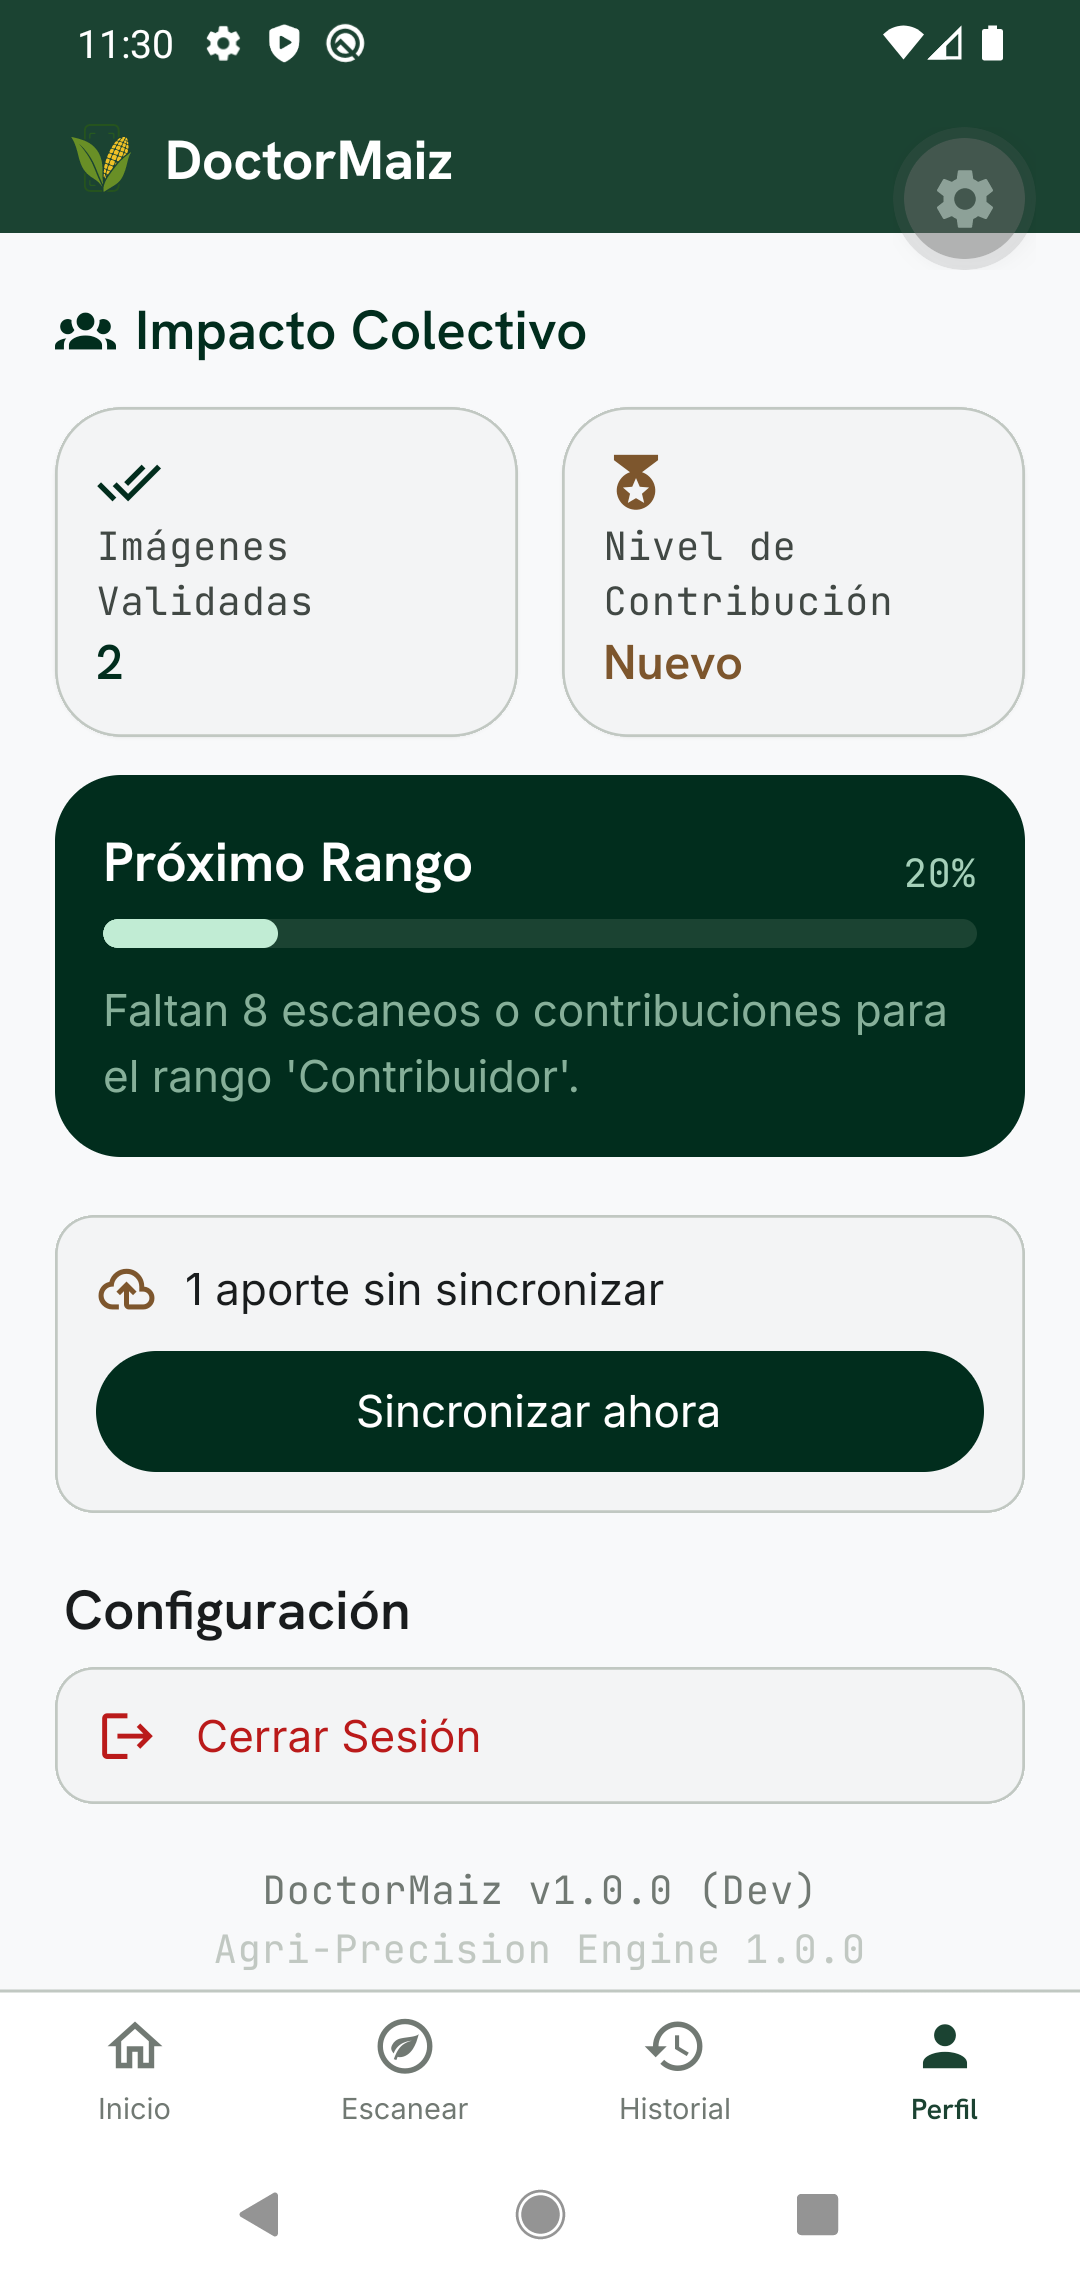
\includegraphics[width=0.46\linewidth]{img/pixel4_profile_guest.png}
    \caption{Pantalla de perfil en Modo Invitado: informa con claridad que puedes escanear y revisar tu historial sin necesidad de registrarte.}
    \label{fig:profile_guest}
\end{figure}

\section{Crear una Cuenta Nueva}
Tener una cuenta te permite sincronizar tus datos cuando llegues a un lugar con Wi-Fi y participar en el proyecto comunitario de mapeo agrícola.

Para registrarte:
\begin{enumerate}
    \item Ve a la pestaña \textbf{Perfil} en la barra inferior y presiona \textbf{Iniciar Sesión}.
    \item En la parte inferior de la pantalla de bienvenida, toca el enlace \textbf{Crear una cuenta nueva}.
    \item Escribe tu nombre completo, tu correo electrónico y define una contraseña segura que recuerdes con facilidad.
    \item Confirma la contraseña en la casilla inferior y presiona el botón verde \textbf{Registrarse}.
\end{enumerate}

\begin{figure}[H]
    \centering
    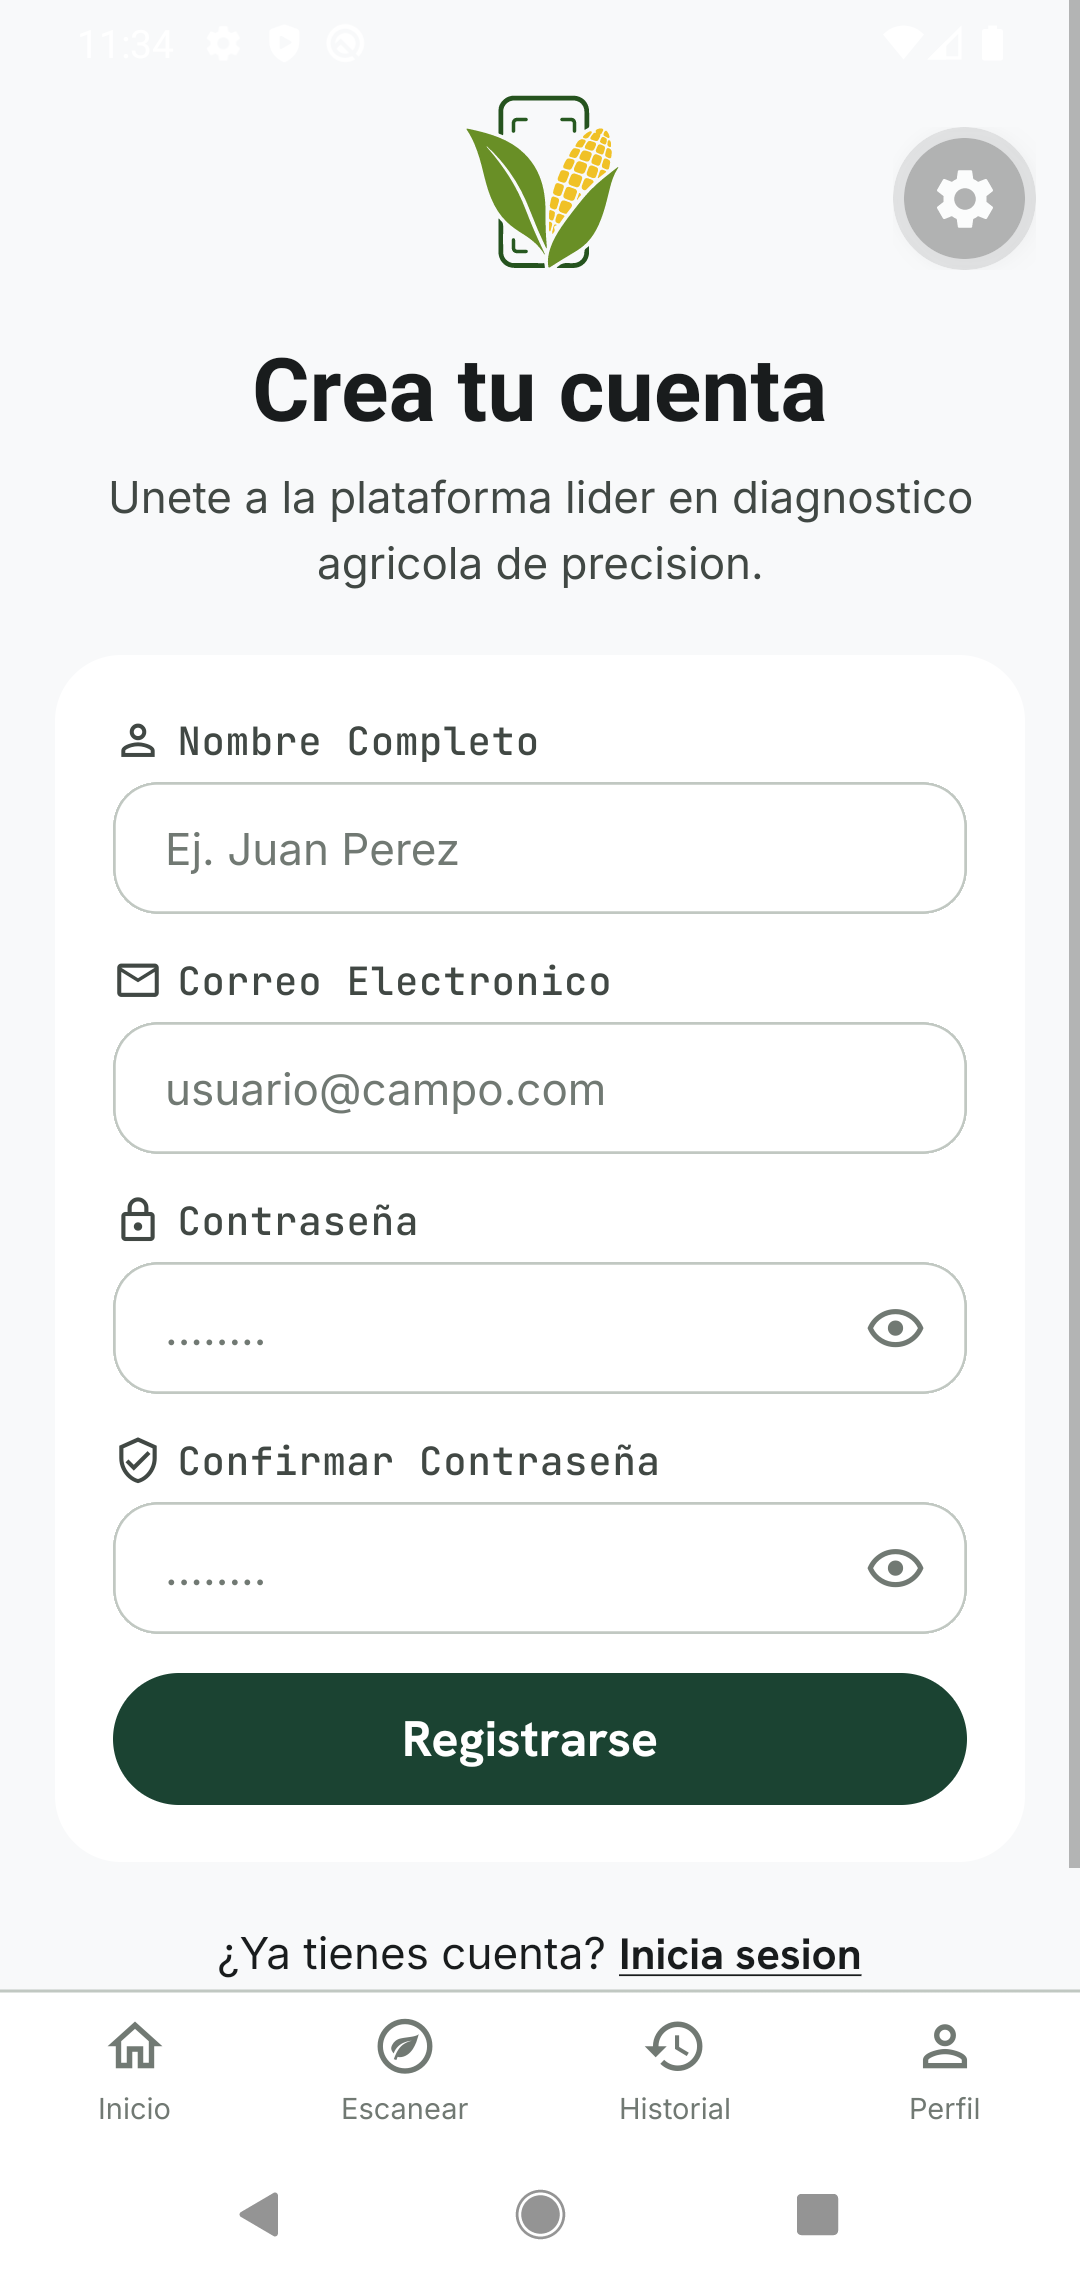
\includegraphics[width=0.46\linewidth]{img/pixel4_register.png}
    \caption{Formulario de registro de nueva cuenta en Doctor Maíz.}
    \label{fig:register_screen}
\end{figure}

\section{Iniciar Sesión y Recuperación de Contraseña}
Si ya te registraste previamente, entra con tu correo y contraseña habituales. 

\begin{figure}[H]
    \centering
    \begin{minipage}{0.48\textwidth}
        \centering
        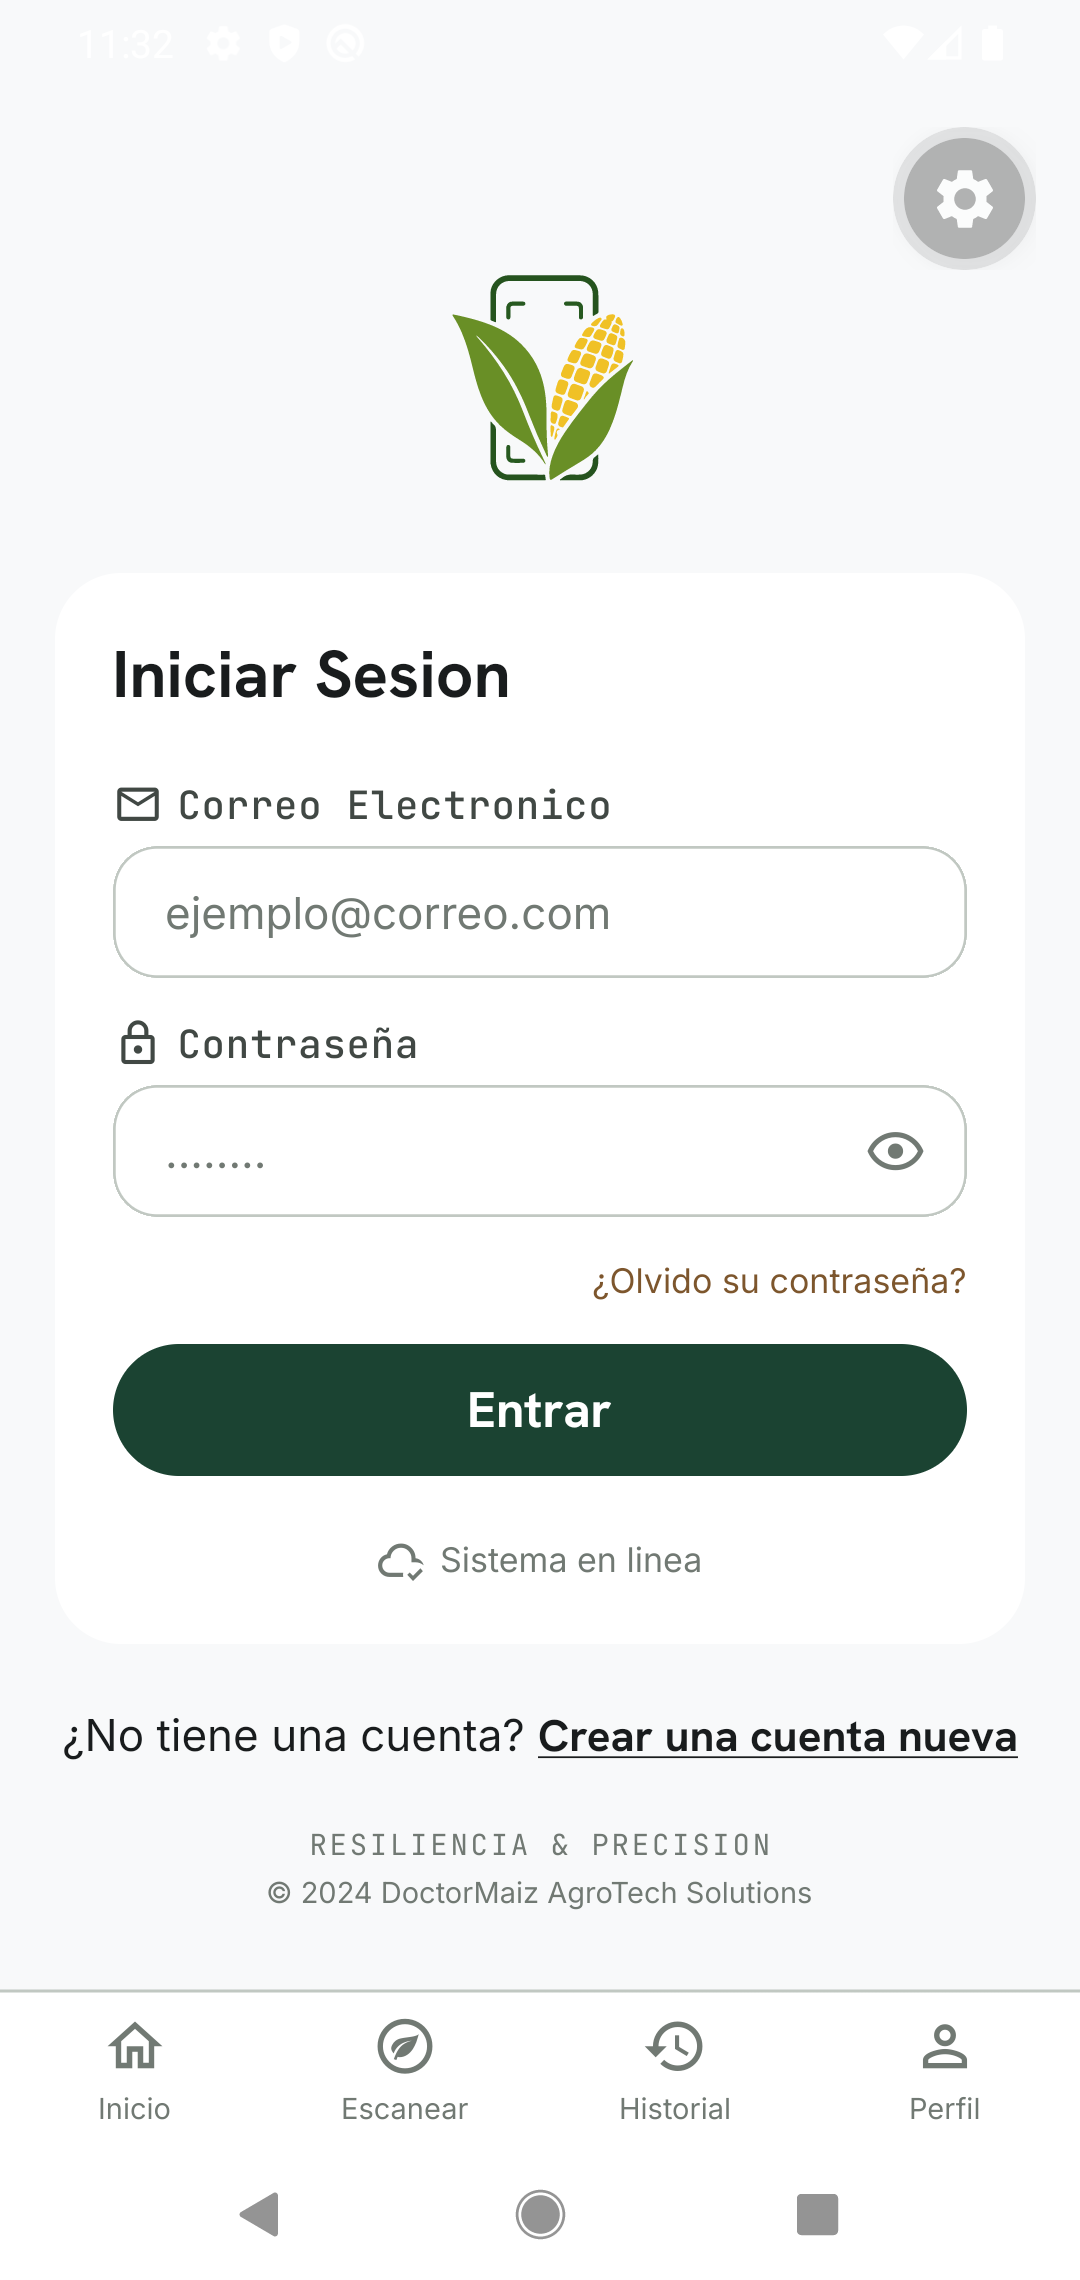
\includegraphics[width=0.92\linewidth]{img/pixel4_login.png}
        \caption{Pantalla de acceso seguro.}
    \end{minipage}
    \hfill
    \begin{minipage}{0.48\textwidth}
        \centering
        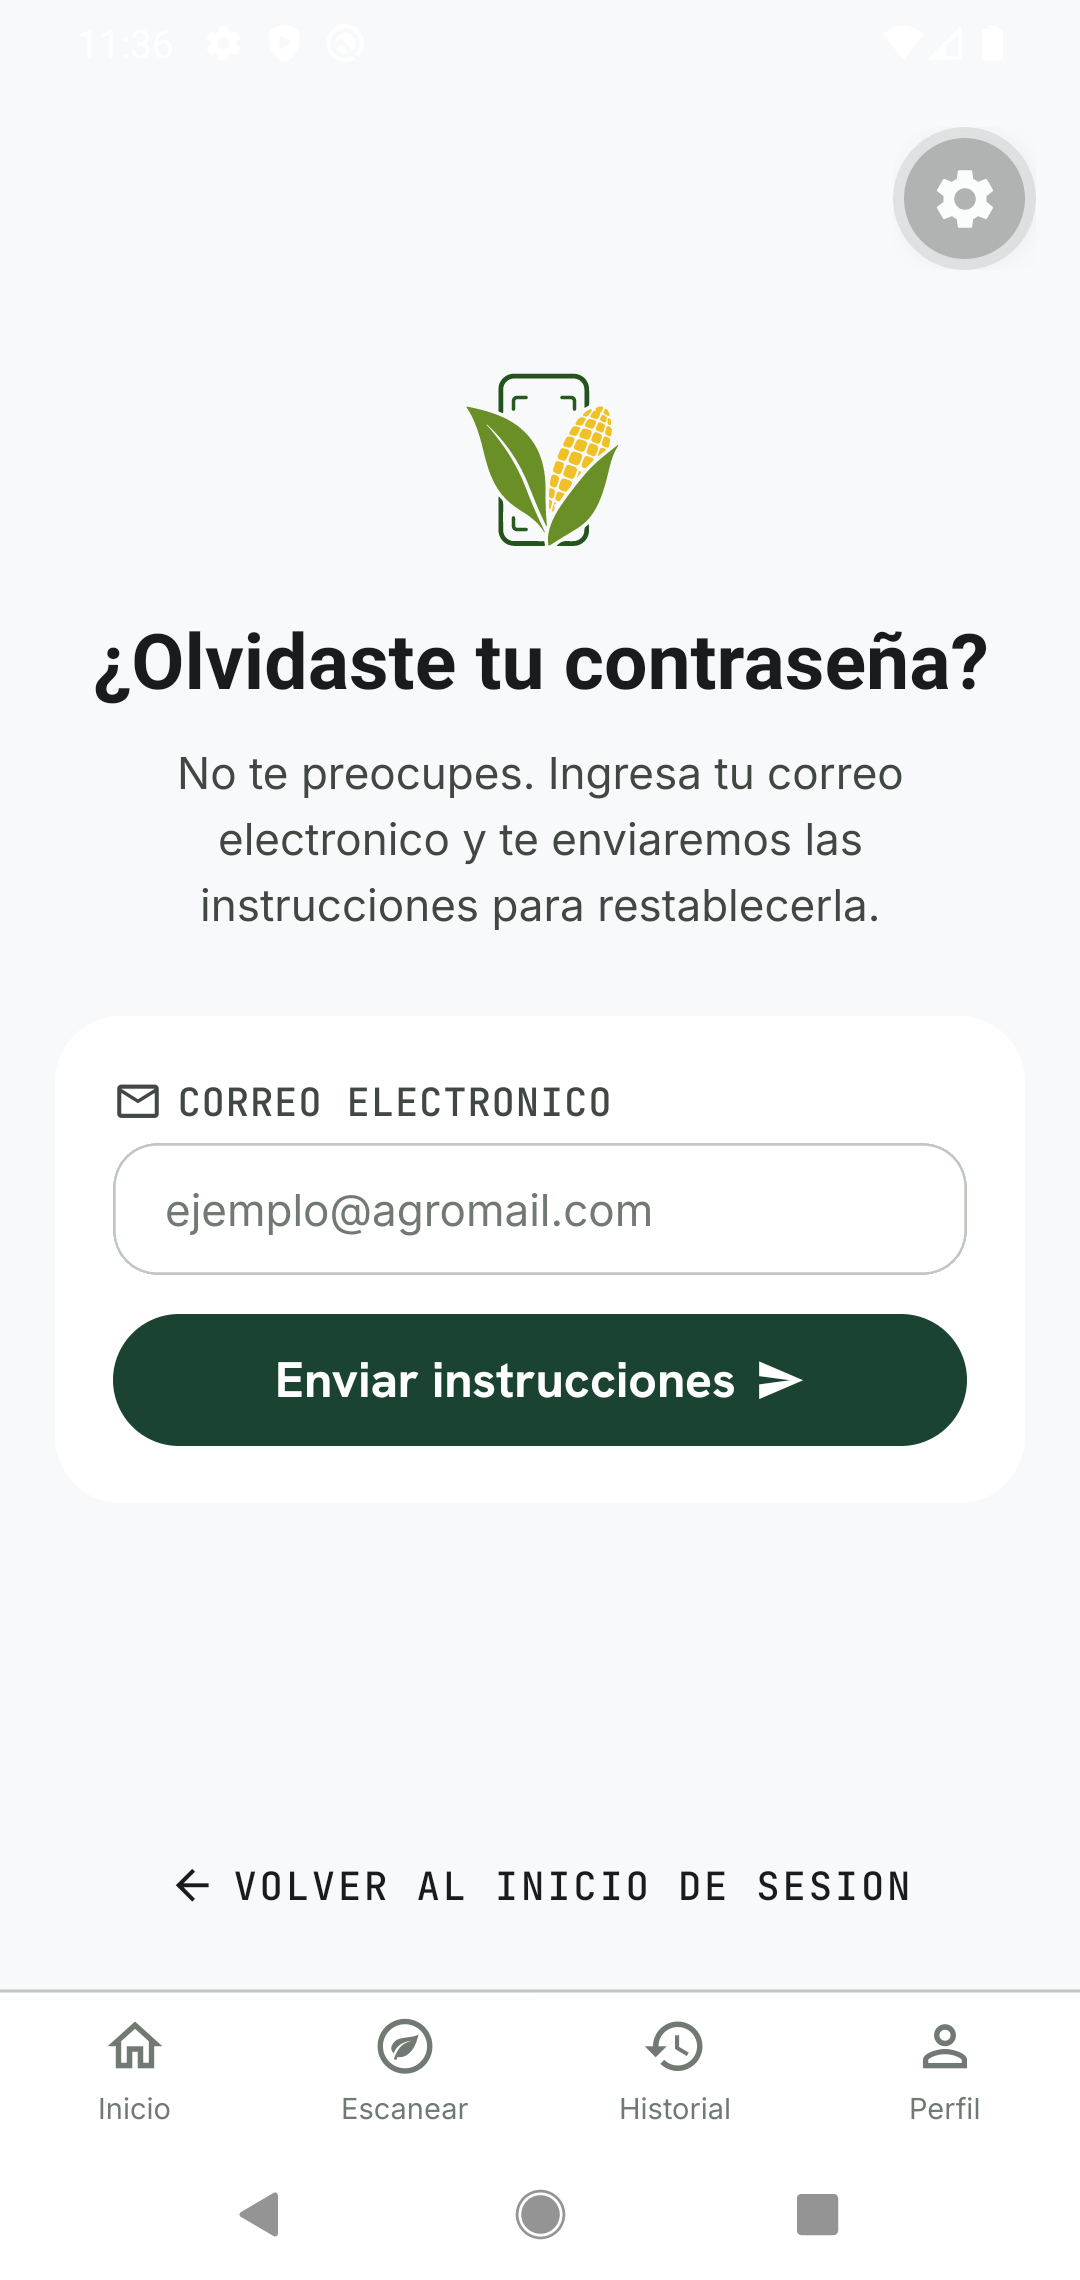
\includegraphics[width=0.92\linewidth]{img/pixel4_forgot_password.png}
        \caption{Recuperación de contraseña.}
    \end{minipage}
\end{figure}

Si olvidaste tu clave, toca sobre \textbf{¿Olvidó su contraseña?}, escribe tu correo electrónico y presiona \textbf{Enviar instrucciones}. Cuando el teléfono tenga conexión, recibirás un mensaje para restablecerla.

% -------------------------------------------------------------
% CAPÍTULO 3: PERFIL DEL PRODUCTOR Y SINCRONIZACIÓN
% -------------------------------------------------------------
\chapter{Perfil del Productor y Sincronización}

La pestaña \textbf{Perfil} concentra tu información como productor, tus logros dentro de la plataforma y el estado de sincronización entre el teléfono y el servidor.

\begin{figure}[H]
    \centering
    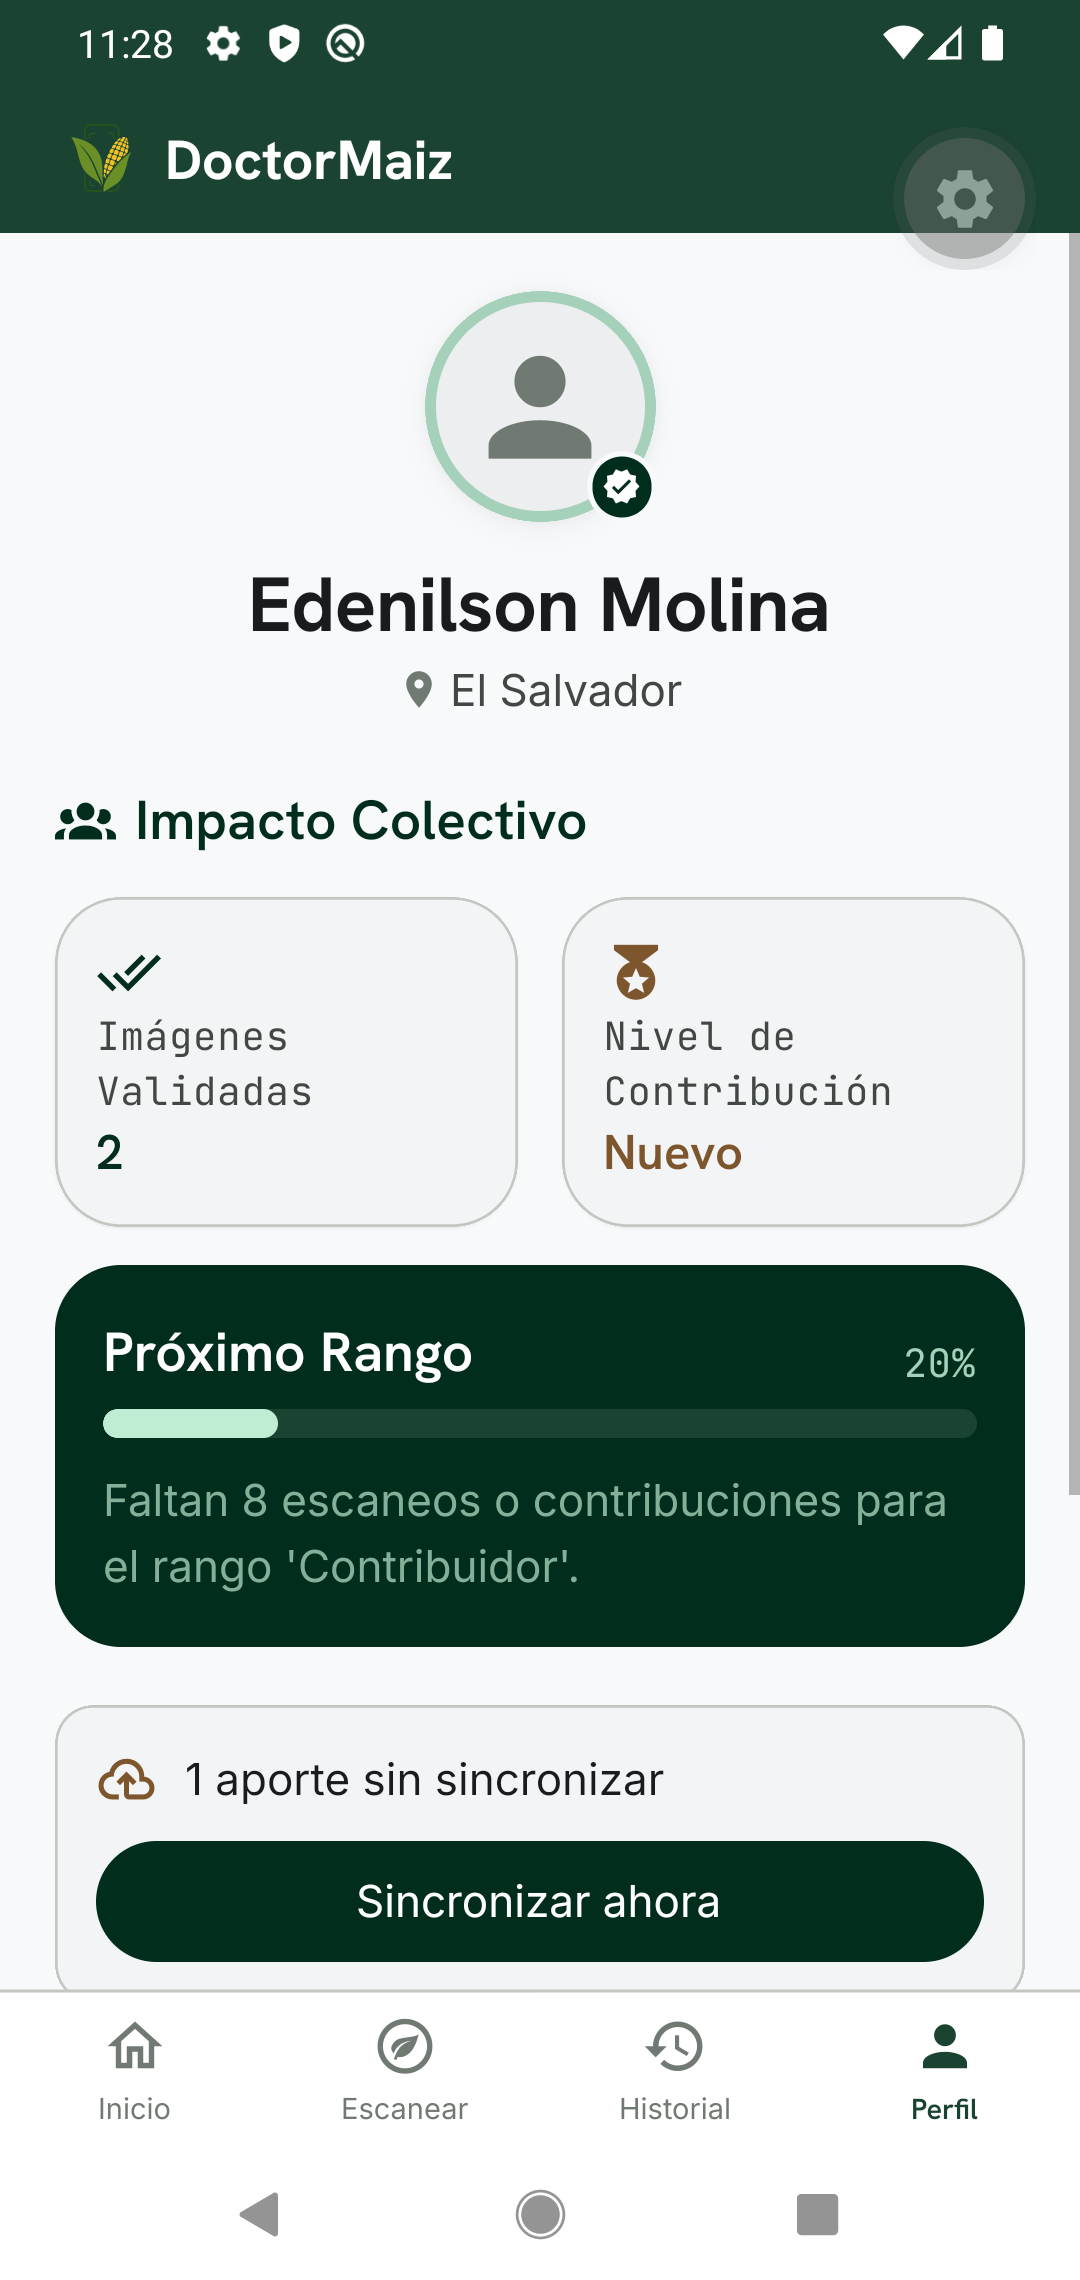
\includegraphics[width=0.46\linewidth]{img/pixel4_profile.png}
    \caption{Perfil de productor con métricas de impacto colectivo y botón de sincronización de aportes.}
    \label{fig:profile_user}
\end{figure}

\section{Impacto Colectivo y Rangos}
Cada vez que recorres tu cultivo y registras plantas sanas o enfermas, estás generando información valiosa para la agricultura de tu región:
\begin{itemize}
    \item \textbf{Imágenes Validadas:} Cantidad de fotografías con diagnóstico confirmado registradas en tu historial.
    \item \textbf{Nivel de Contribución:} Reconocimiento a tu constancia en el monitoreo (\textit{Nuevo}, \textit{Contribuidor}, \textit{Experto}).
    \item \textbf{Barra de Próximo Rango:} Te muestra cuántos escaneos te faltan para subir de nivel.
\end{itemize}

\section{Cómo Sincronizar tus Muestras}
En el campo, el teléfono almacena cada escaneo en una base de datos local rápida (\texttt{SQLite} con \texttt{WatermelonDB}). Cuando vuelvas a casa, a la bodega o a una zona con cobertura celular:
\begin{enumerate}
    \item Abre la pestaña \textbf{Perfil}.
    \item Verás un aviso que indica cuántos aportes están pendientes por subir (por ejemplo: \textit{«1 aporte sin sincronizar»}).
    \item Presiona el botón verde \textbf{Sincronizar ahora}.
    \item En pocos segundos, tus datos quedarán respaldados de forma segura en la nube.
\end{enumerate}

\section{Cerrar Sesión}
Al final de la pantalla de perfil encontrarás el botón rojo \textbf{Cerrar Sesión}. Esto es útil si vas a prestar el teléfono a otro productor para que trabaje con su propia cuenta, o si prefieres volver al Modo Invitado.

% -------------------------------------------------------------
% CAPÍTULO 4: PANTALLA PRINCIPAL Y MONITOREO DEL CLIMA
% -------------------------------------------------------------
\chapter{Pantalla Principal y Monitoreo del Clima}

La pantalla de **Inicio** es tu centro de operaciones cada mañana antes de salir al lote. Está diseñada para darte una lectura rápida de las condiciones del ambiente y el estado general de tu siembra.

\begin{figure}[H]
    \centering
    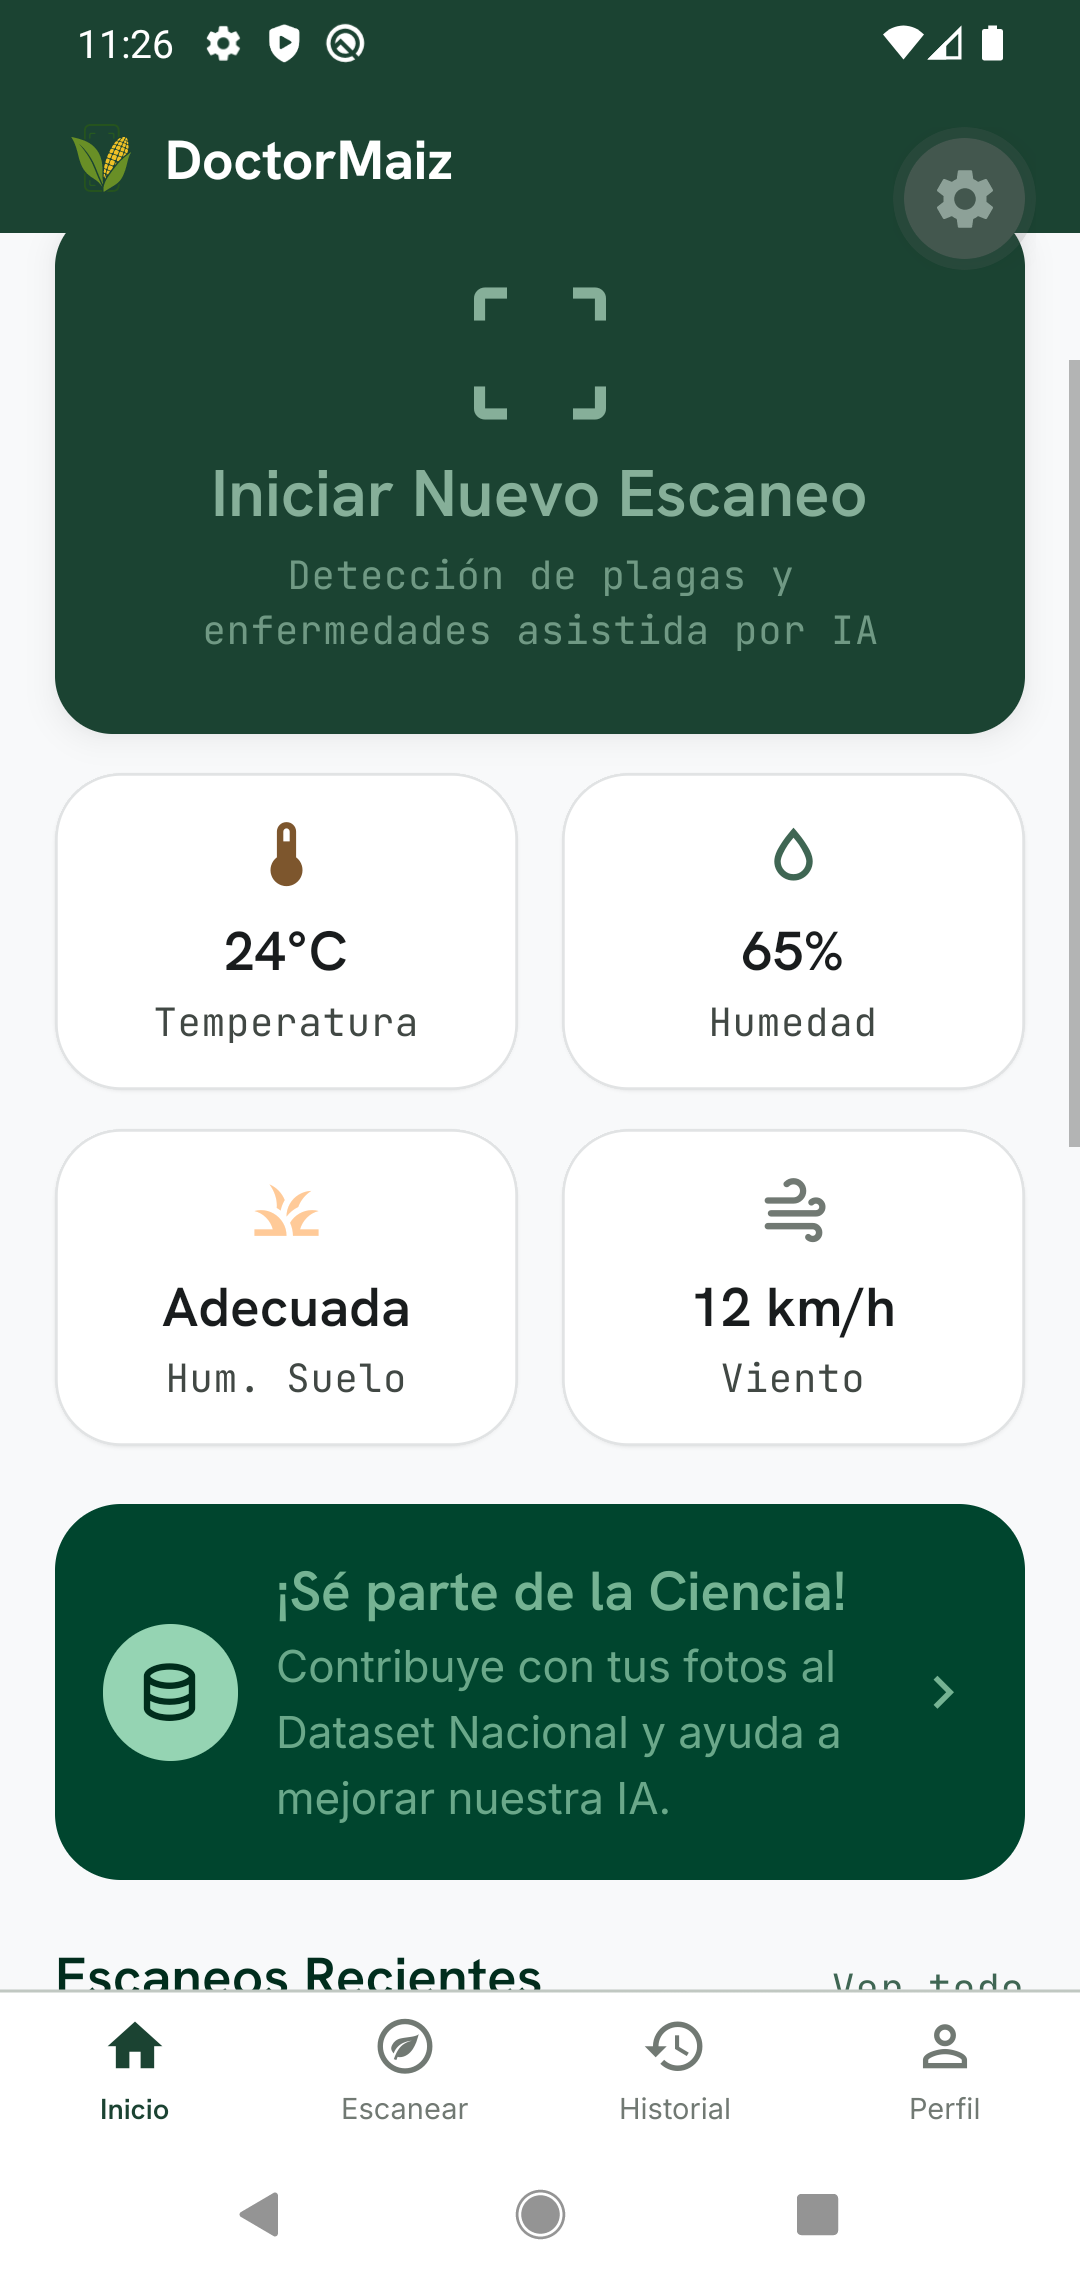
\includegraphics[width=0.46\linewidth]{img/pixel4_home_top.png}
    \caption{Pantalla de Inicio con indicadores microclimáticos en tiempo real y acceso directo a nuevo escaneo.}
    \label{fig:home_top}
\end{figure}

\section{Lectura de Variables Agroclimáticas}
En la parte superior encontrarás cuatro tarjetas con datos fundamentales:
\begin{itemize}
    \item \textbf{Temperatura ($^\circ\text{C}$):} Calor actual en la zona. Temperaturas entre 20 y 28 $^\circ\text{C}$ con humedad alta favorecen la germinación de esporas de hongos como la roya.
    \item \textbf{Humedad Relativa (\%):} Porcentaje de vapor de agua en el aire. Si supera el 80\% de manera prolongada, se activa el riesgo de enfermedades foliares.
    \item \textbf{Humedad del Suelo:} Te indica si el suelo se encuentra en nivel \textit{Adecuado}, \textit{Seco} o con \textit{Exceso de Agua}, ayudándote a regular los turnos de riego o drenaje.
    \item \textbf{Viento (km/h):} Velocidad del aire. Vientos mayores a 15 km/h desaconsejan las aplicaciones foliares porque el viento desvía la gota y acelera la dispersión de esporas entre parcelas.
\end{itemize}

\section{Acceso Rápido al Escáner}
El recuadro grande en color verde oscuro titulado **«Iniciar Nuevo Escaneo»** te lleva directamente a la cámara de diagnóstico sin tener que buscar en ningún submenú.

% -------------------------------------------------------------
% CAPÍTULO 5: EL ESCÁNER Y LA CÁMARA EN EL SURCO
% -------------------------------------------------------------
\chapter{El Escáner: Captura y Diagnóstico en el Surco}

El corazón de Doctor Maíz es su cámara inteligente. A diferencia de las aplicaciones que requieren enviar la foto a un servidor en internet, aquí la red neuronal vive en el teléfono y te da el resultado de inmediato.

\begin{figure}[H]
    \centering
    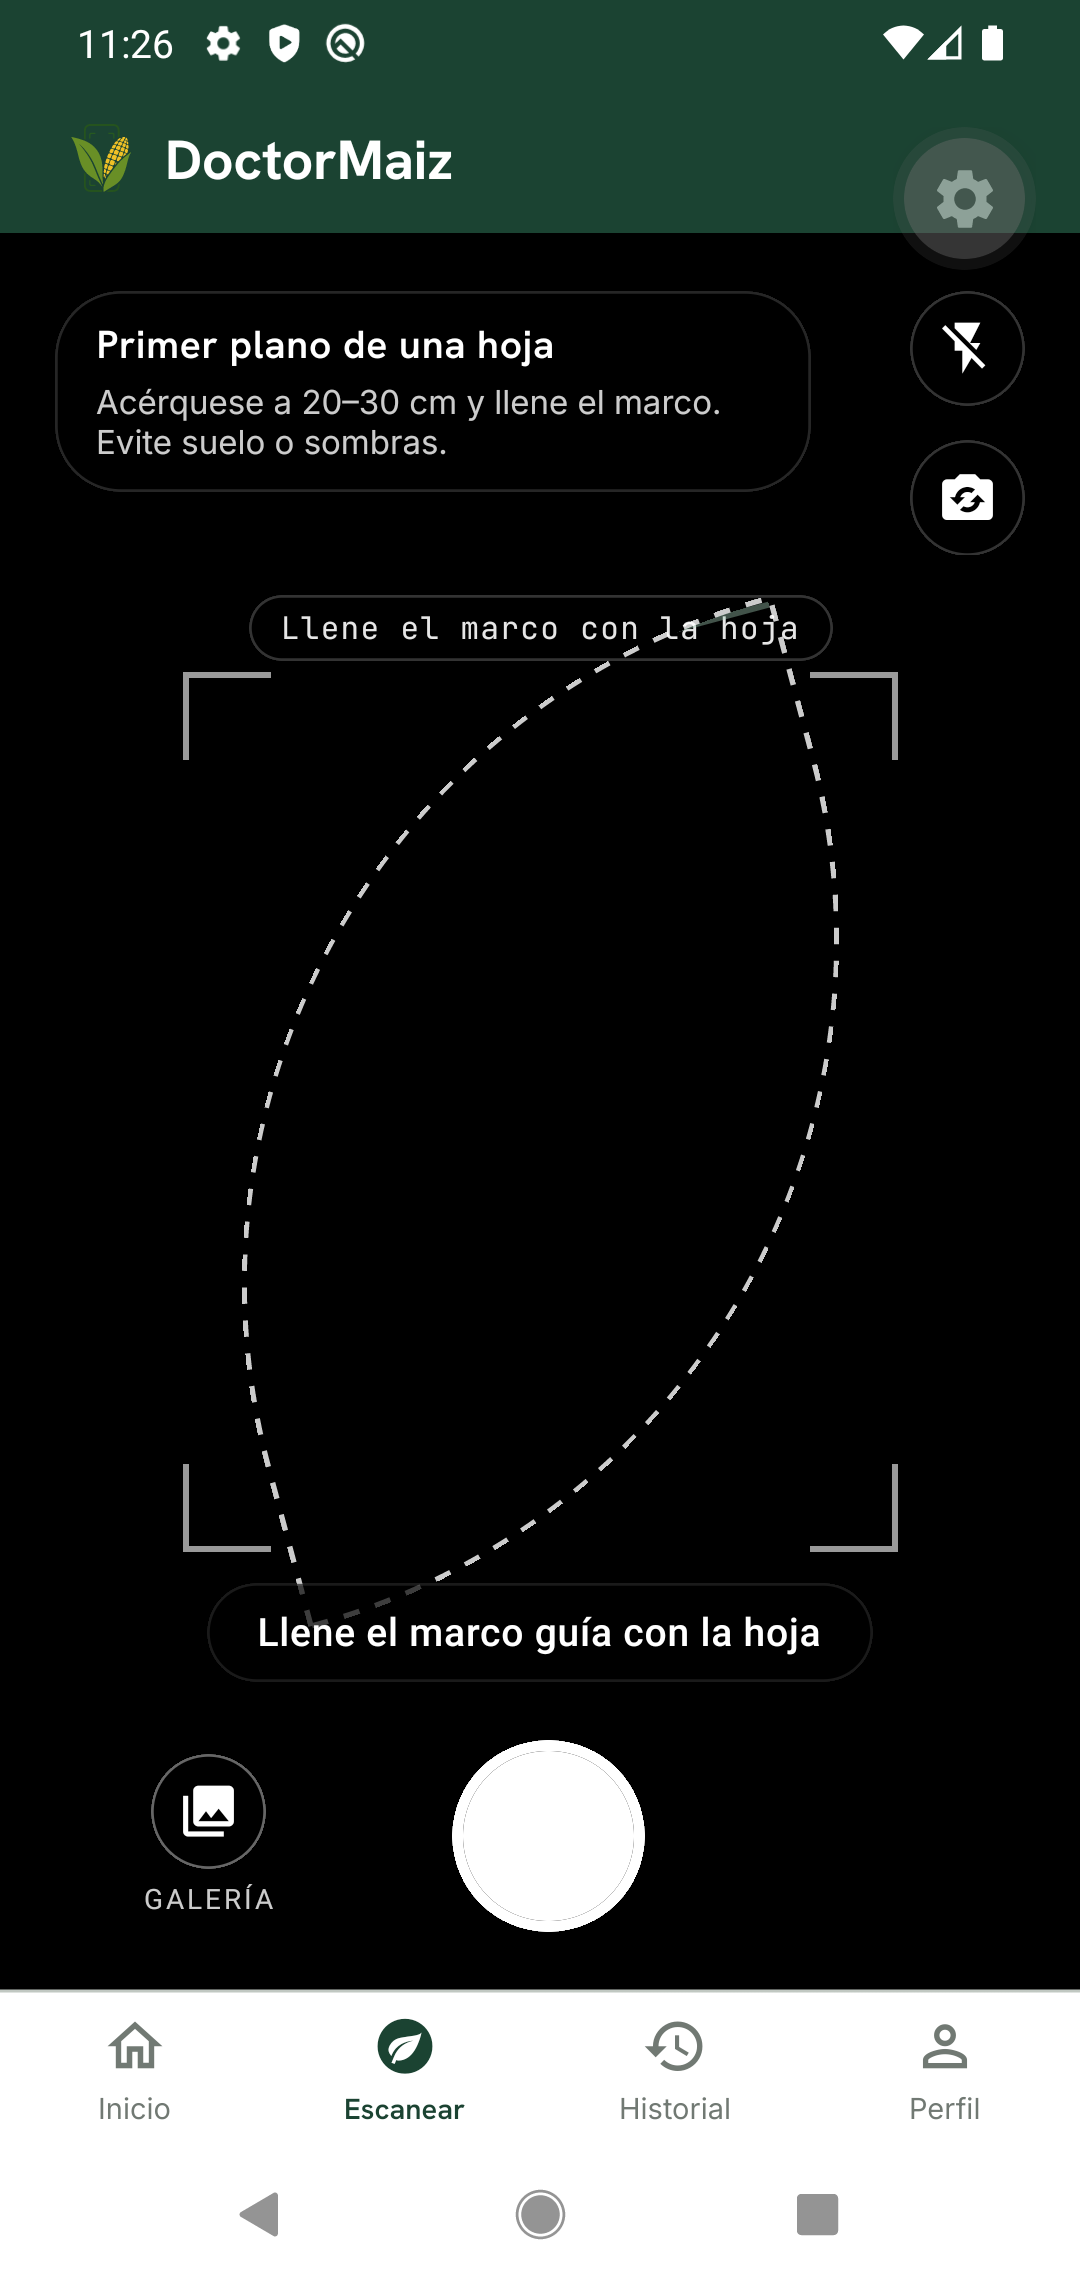
\includegraphics[width=0.46\linewidth]{img/pixel4_camera.png}
    \caption{Visor de la cámara con la silueta guía de la hoja de maíz y recomendaciones de encuadre.}
    \label{fig:camera_view}
\end{figure}

\section{Cómo Encuadrar la Hoja con la Retícula}
Cuando abres el escáner, verás en pantalla una silueta punteada con forma de hoja de maíz:
\begin{enumerate}
    \item Elige una hoja del tercio medio de la planta (ni la más vieja que toca el suelo ni el cogollo tierno, a menos que busques gusano cogollero).
    \item Coloca el lente a una distancia de **20 a 30 centímetros** de la hoja.
    \item Haz que la lámina de la hoja llene el marco punteado de la pantalla.
    \item Toca sobre el síntoma o mancha para que la cámara enfoque con nitidez.
    \item Presiona el botón circular blanco del centro para tomar la fotografía.
\end{enumerate}

\begin{campotip}
    \textbf{Cómo evitar que el sol engañe a la cámara:} No tomes fotos a contraluz. Si el sol de mediodía es muy fuerte, párate de espaldas al sol para que tu propio cuerpo proyecte una sombra suave y pareja sobre la hoja. Así los colores saldrán reales y la cámara no se encandilará.
\end{campotip}

\section{El Detector Fuera de Dominio (Fotos Inválidas)}
Si sin querer presionas el botón apuntando al suelo, a tus botas, a una persona, a una maleza desconocida o a un vehículo, la app te avisará que la imagen es **«No Reconocida»**. Esto evita que el sistema te dé un diagnóstico inventado cuando la foto no corresponde a una hoja de maíz.

\section{Uso de Fotos de la Galería}
Si tomaste fotos temprano con la cámara estándar de tu teléfono o si un colega te mandó una foto por mensajería, toca el botón **Galería** (a la izquierda del disparador blanco) para cargar la imagen y recibir el diagnóstico de inmediato.

% -------------------------------------------------------------
% CAPÍTULO 6: RESULTADOS Y GUÍA DE SEVERIDAD EN 3 NIVELES
% -------------------------------------------------------------
\chapter{Interpretación de Resultados y Severidad}

Al presionar el disparador, en menos de un segundo verás la pantalla de detalle del escaneo.

\begin{figure}[H]
    \centering
    \begin{minipage}{0.48\textwidth}
        \centering
        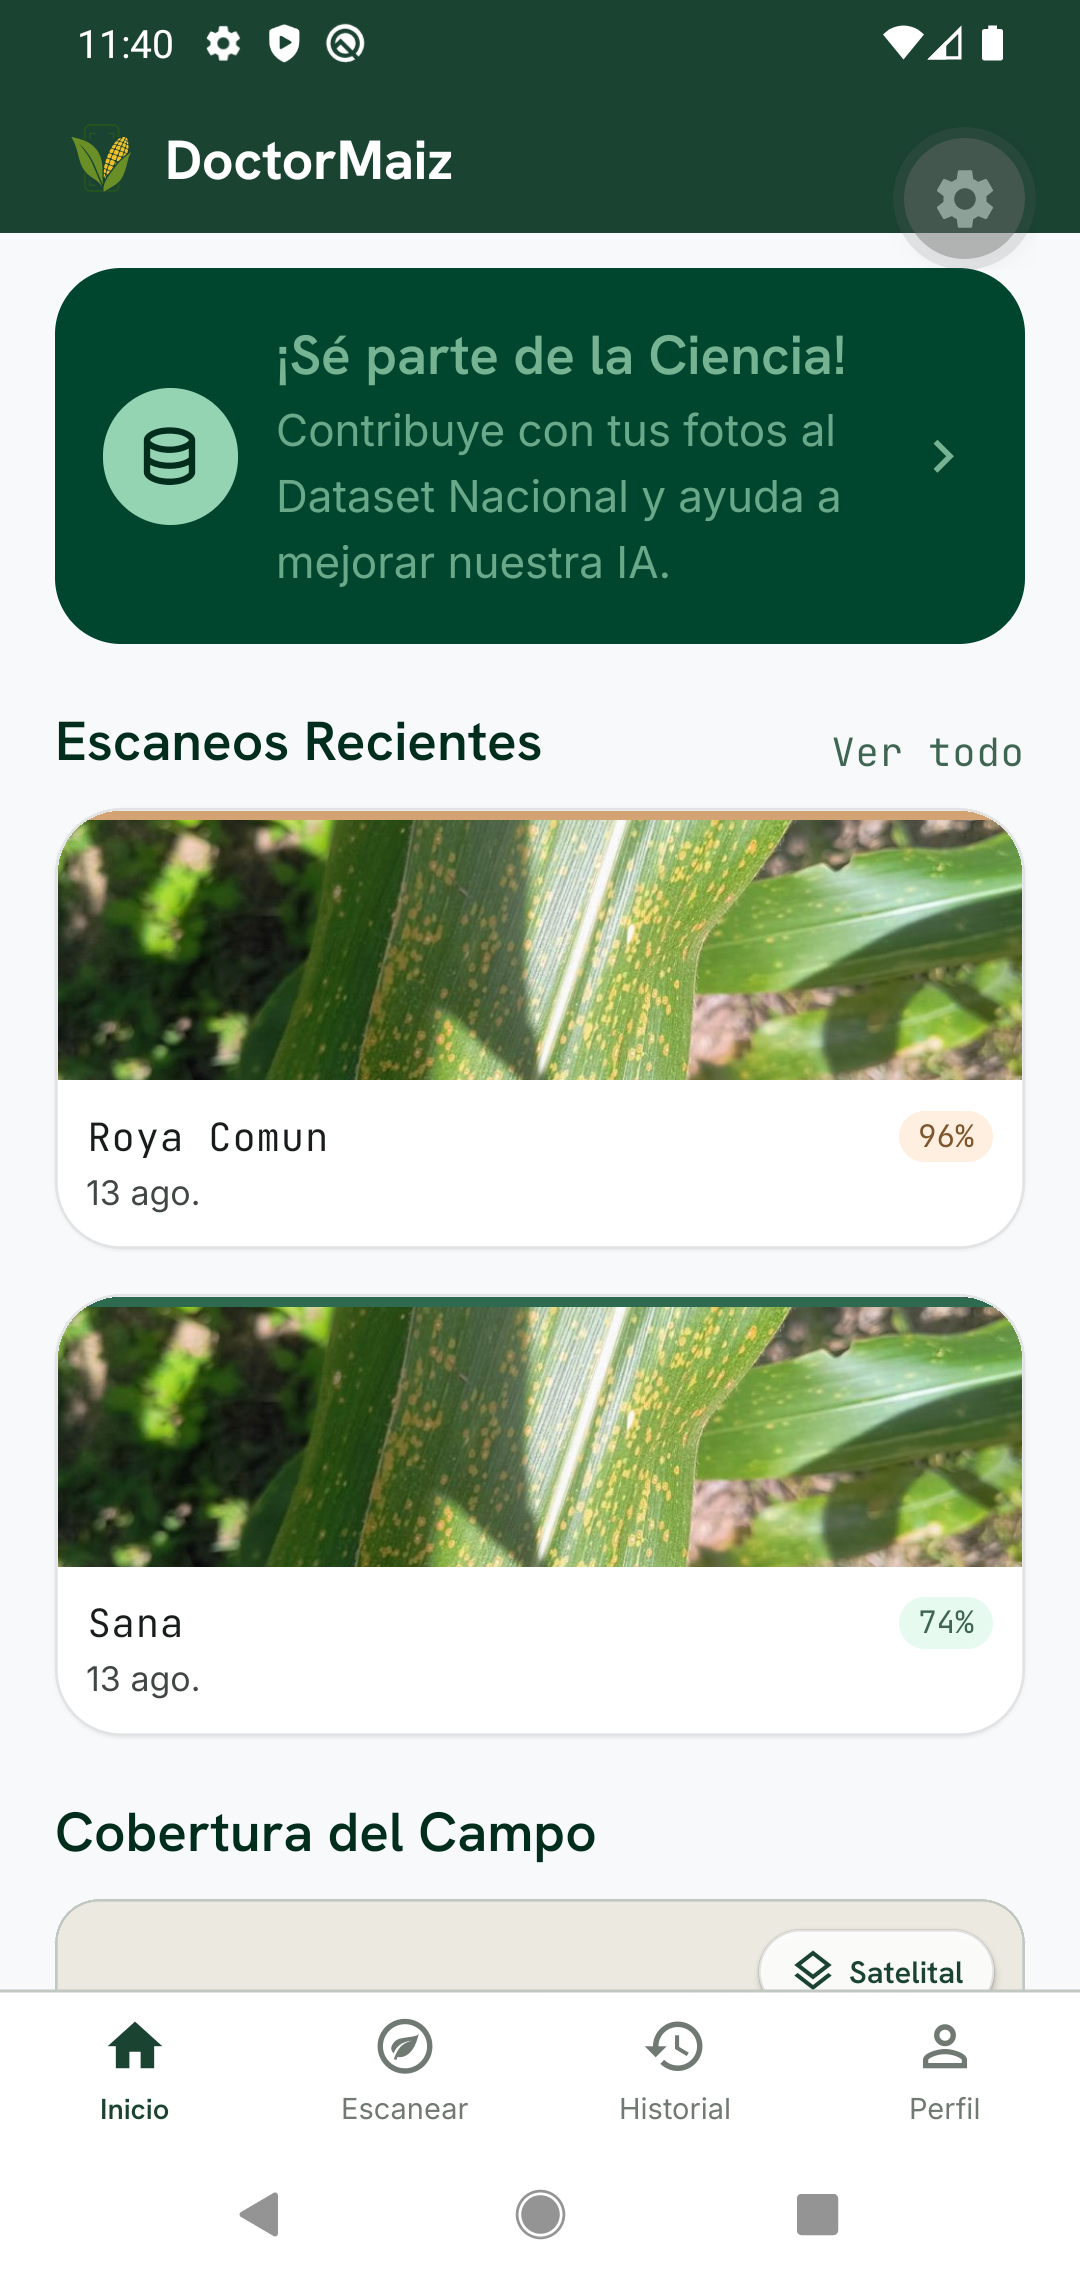
\includegraphics[width=0.92\linewidth]{img/pixel4_detail_scan.png}
        \caption{Resultado de diagnóstico con foto y condiciones registradas.}
    \end{minipage}
    \hfill
    \begin{minipage}{0.48\textwidth}
        \centering
        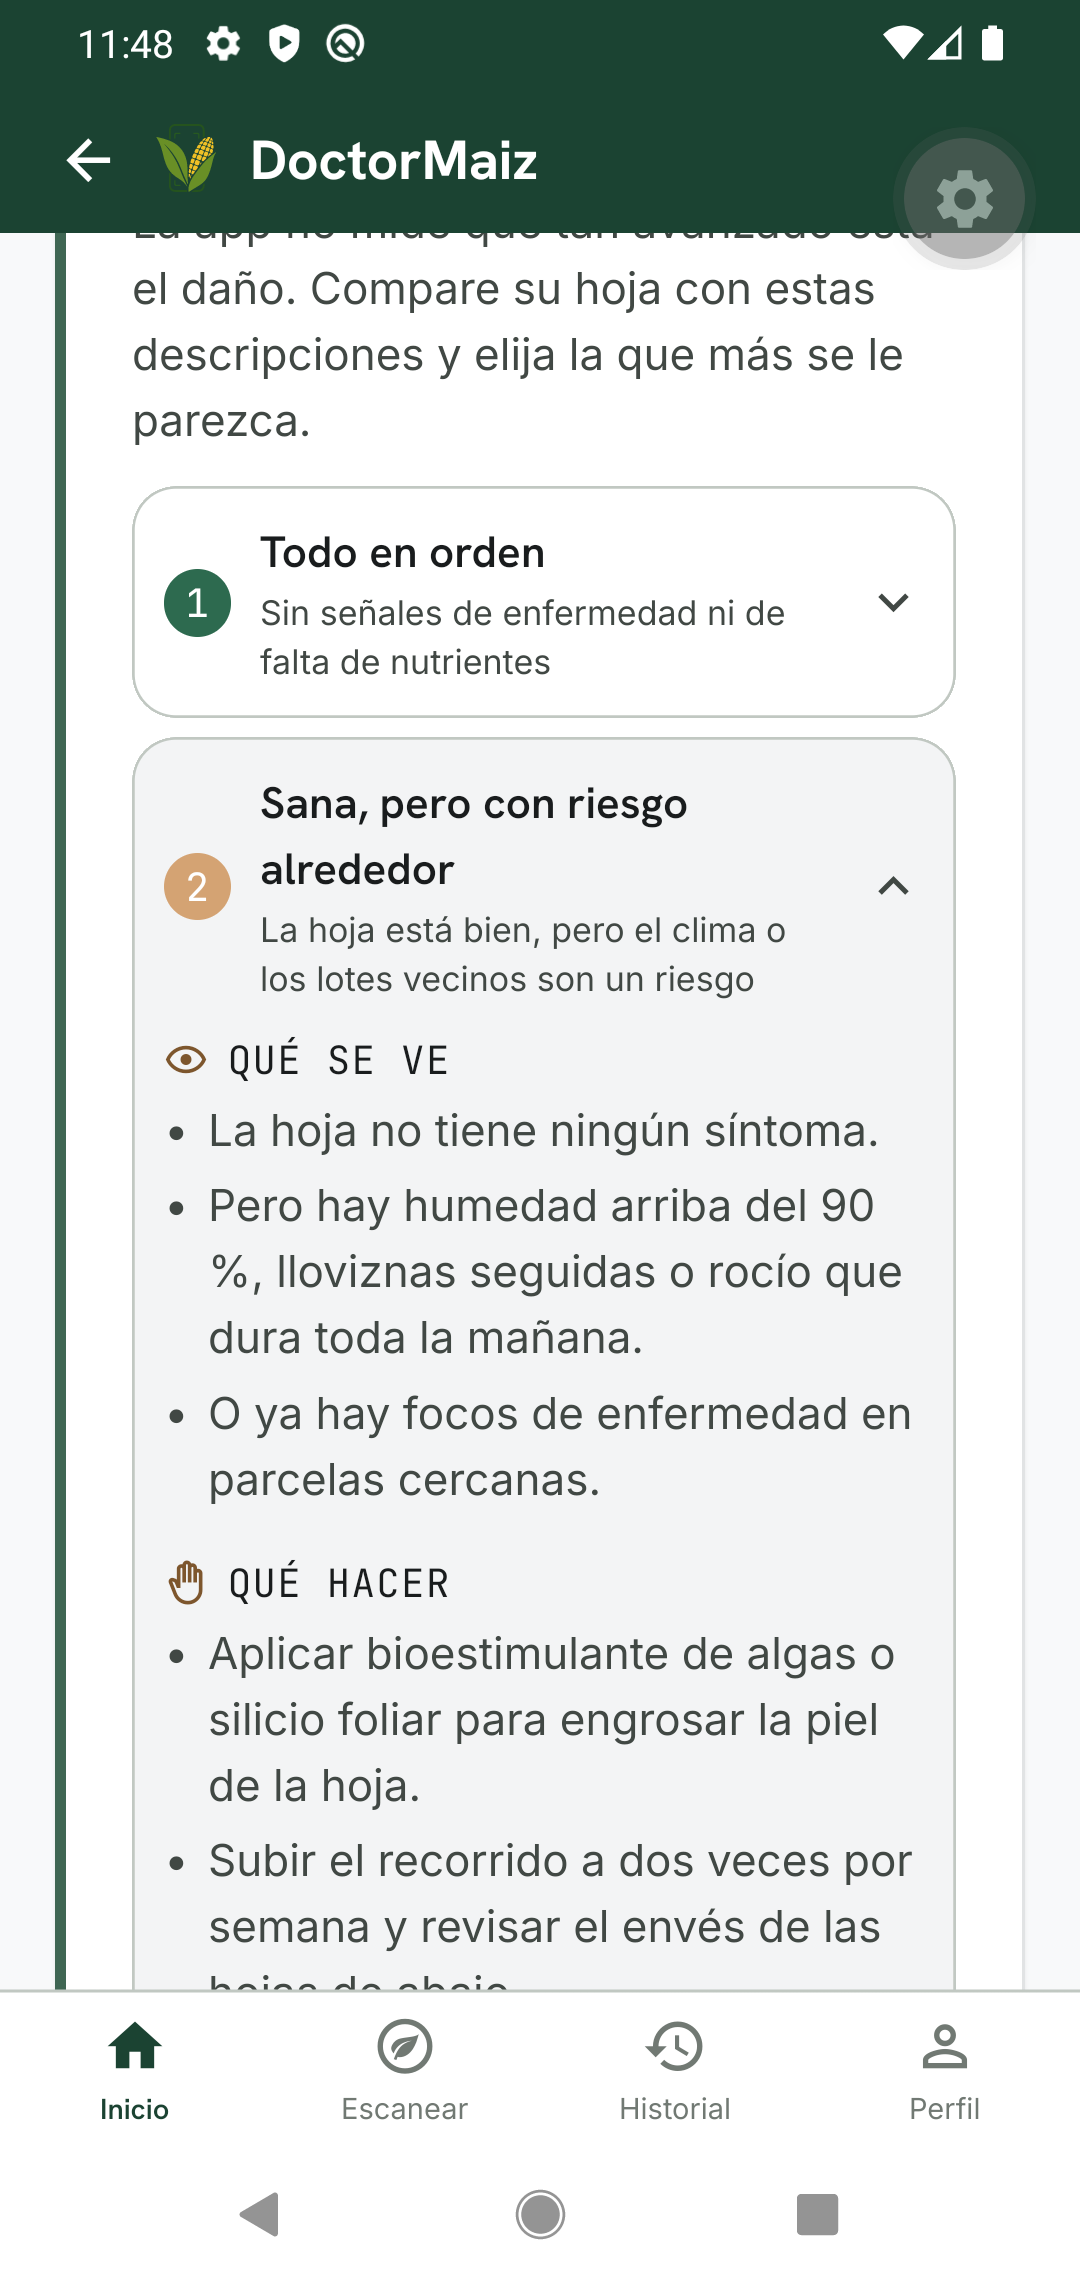
\includegraphics[width=0.92\linewidth]{img/pixel4_detail_accordion.png}
        \caption{Guía de Severidad desplegada con síntomas y acciones.}
    \end{minipage}
\end{figure}

\section{Cómo Leer el Diagnóstico}
La pantalla te muestra tres datos principales:
\begin{enumerate}
    \item \textbf{Nombre de la Condición:} Te indica el problema detectado (por ejemplo: \textit{Roya Común}, \textit{Gusano Cogollero}, \textit{Deficiencia de Nitrógeno} o \textit{Sana}).
    \item \textbf{Porcentaje de Confianza:} Qué tan seguro está el modelo de su predicción (por ejemplo: \textit{96\% de certeza}).
    \item \textbf{Datos del Momento:} Fecha, hora y valores climáticos registrados en ese instante.
\end{enumerate}

\section{¿Por qué una Guía de Severidad y no un Porcentaje Inventado?}
Muchos programas intentan predecir qué tan grave es el daño calculando porcentajes automáticos que casi siempre fallan en campo, porque dos manchas pequeñas de roya en una hoja joven son más peligrosas que diez manchas secas en una hoja vieja a punto de cosechar.

Doctor Maíz utiliza una filosofía honesta: **la app te dice qué tiene la planta, y tú decides qué tan avanzada está comparando con descripciones claras**.

\section{Los 3 Niveles del Acordeón}
Al tocar el bloque desplegable verás tres niveles:

\begin{description}
    \item[\textcolor{MaizPrimary}{\textbf{Nivel 1: Apenas empieza (Leve)}}]
    \begin{itemize}
        \item \textbf{Qué se ve:} Muy pocas manchas o puntitos aislados (menos del 2\% de la hoja comprometida). La mayor parte de la hoja está verde y firme.
        \item \textbf{Qué hacer:} No gastes en venenos fuertes. Es el momento perfecto para aplicar preventivos biológicos como *Bacillus subtilis* o silicio foliar para endurecer la cutícula de la hoja.
    \end{itemize}

    \item[\textcolor{MaizGold}{\textbf{Nivel 2: Ya se está extendiendo (Moderado)}}]
    \begin{itemize}
        \item \textbf{Qué se ve:} Las manchas empiezan a juntarse, cubriendo entre el 5\% y el 15\% de la superficie. Ya hay hojas bajas amarillentas.
        \item \textbf{Qué hacer:} Realiza aplicaciones dirigidas a los focos infectados. Revisa el lote dos veces por semana para vigilar que no suba hacia la hoja de la mazorca.
    \end{itemize}

    \item[\textcolor{MaizRed}{\textbf{Nivel 3: Daño grave (Crítico)}}]
    \begin{itemize}
        \item \textbf{Qué se ve:} Más del 15\% o 20\% de la lámina está seca, perforada o quemada. Hay presencia abundante de aserrín o pústulas reventadas.
        \item \textbf{Qué hacer:} Requiere acción inmediata para proteger las plantas vecinas sanas. Consulta con el técnico de confianza para decidir si amerita una intervención de choque antes de que afecte el llenado de grano.
    \end{itemize}
\end{description}

% -------------------------------------------------------------
% CAPÍTULO 7: CATÁLOGO DE ENFERMEDADES Y DEFICIENCIAS
% -------------------------------------------------------------
\chapter{Catálogo de Enfermedades y Deficiencias}

El modelo de Doctor Maíz fue entrenado con más de 31,000 fotografías reales de campo y reconoce nueve situaciones agrícolas cotidianas:

\begin{table}[H]
\centering
\small
\begin{tabularx}{\linewidth}{>{\bfseries\raggedright\arraybackslash}p{3.6cm} >{\raggedright\arraybackslash}p{4.2cm} >{\raggedright\arraybackslash}X}
\toprule
\textbf{Condición} & \textbf{Causa Principal} & \textbf{Cómo Reconocerla en el Campo} \\
\midrule
Hoja Sana & Planta vigorosa & Verde parejo, venas enteras, textura elástica sin mordeduras. \\
\addlinespace
Roya Común & Hongo (\textit{Puccinia sorghi}) & Granos o pústulas cafés o rojizas que sueltan polvillo en ambas caras de la hoja. \\
\addlinespace
Tizón Foliar del Norte & Hongo (\textit{Exserohilum turcicum}) & Manchas largas en forma de puro o canoa, color verde grisáceo que luego se secan. \\
\addlinespace
Mancha por Cercospora & Hongo (\textit{Cercospora zeae-maydis}) & Manchas rectangulares angostas, frenadas entre las nervaduras de la hoja. \\
\addlinespace
Necrosis Letal & Complejo de virus (MLN) & Amarillamiento en mosaico, hojas de arriba deformadas y muerte descendente. \\
\addlinespace
Gusano Cogollero & Oruga (\textit{Spodoptera frugiperda}) & Hojas deshilachadas, perforaciones en ventana y excremento como aserrín en el cogollo. \\
\addlinespace
Falta de Nitrógeno & Nutrición insuficiente (N) & Amarillamiento que empieza en la punta y avanza en forma de ``V'' por el centro. \\
\addlinespace
Falta de Fósforo & Nutrición insuficiente (P) & Hojas bajas con tonalidades moradas o violáceas en las orillas, tallos delgados. \\
\addlinespace
Falta de Potasio & Nutrición insuficiente (K) & Bordes exteriores de las hojas quemados y secos, mientras el centro sigue verde. \\
\bottomrule
\end{tabularx}
\caption{Guía rápida de identificación visual en campo.}
\label{tab:catalogo_resumen}
\end{table}

\begin{agronote}
    \textbf{Diferencia entre falta de nutrientes y ataque de hongos:} Las deficiencias nutricionales suelen ser parejas en muchas plantas del mismo surco o mancha de suelo. En cambio, los hongos y gusanos casi siempre empiezan en una o dos plantas aisladas que forman pequeños focos circulares.
\end{agronote}

% -------------------------------------------------------------
% CAPÍTULO 8: MAPA DE COBERTURA Y CARTOGRAFÍA DE PARCELAS
% -------------------------------------------------------------
\chapter{Mapa de Cobertura y Cartografía del Lote}

En la parte inferior de la pantalla de inicio encontrarás el **Mapa de Cobertura**, que ubica cada planta escaneada con un punto sobre el terreno.

\begin{figure}[H]
    \centering
    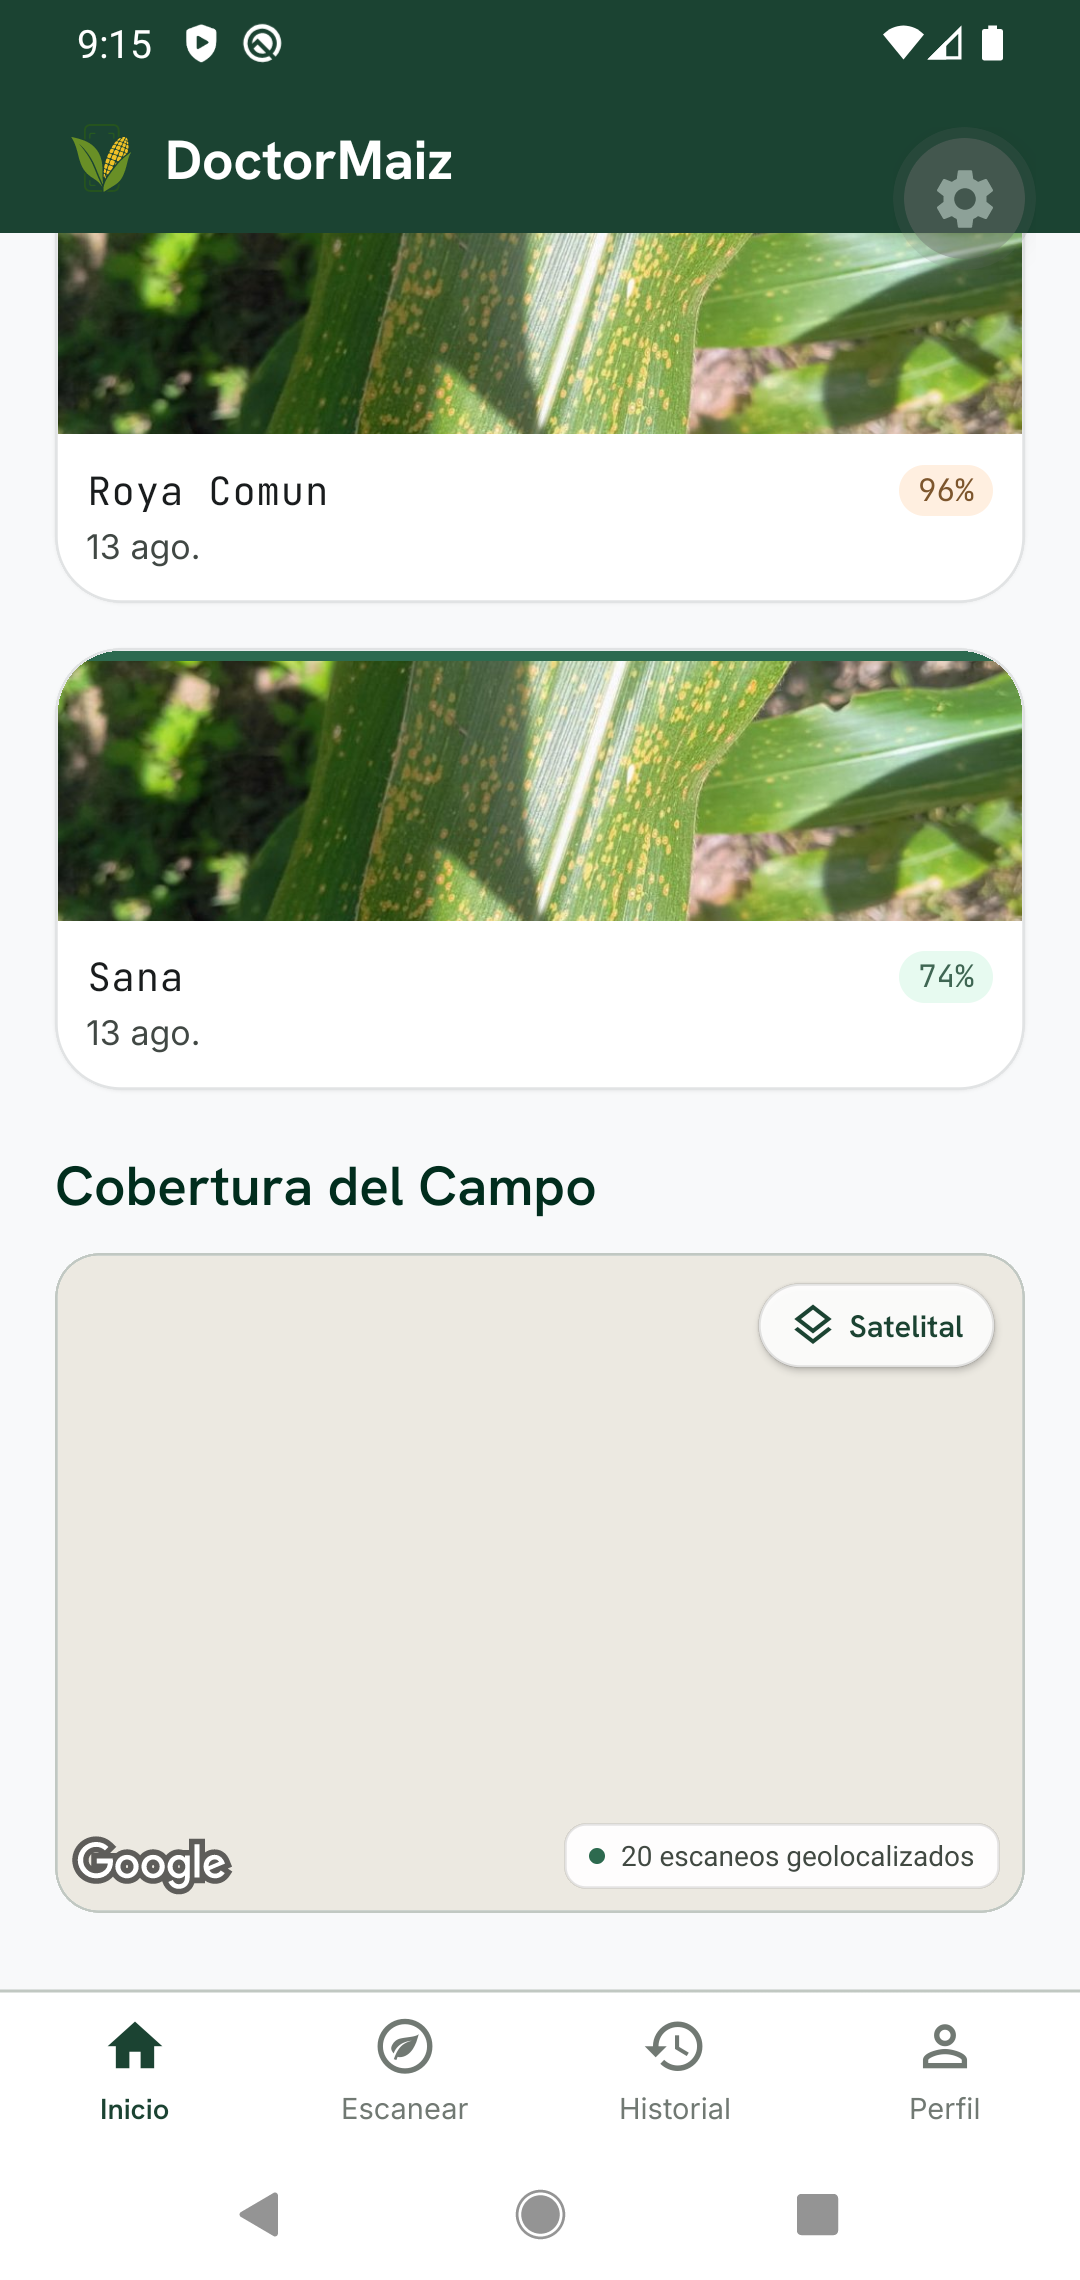
\includegraphics[width=0.58\linewidth]{img/map_screen.png}
    \caption{Mapa de Cobertura en la pantalla principal: muestra los pines geolocalizados en el lote y el conmutador Satelital.}
    \label{fig:map_coverage}
\end{figure}

\section{Código de Colores de los Pines}
Cada marcador en el mapa te indica de un vistazo la gravedad de la zona:
\begin{itemize}
    \item \textbf{Pines Verdes:} Hojas sanas o con problemas muy leves.
    \item \textbf{Pines Amarillos o Mostaza:} Plantas con deficiencias de nutrientes o enfermedades moderadas.
    \item \textbf{Pines Rojos:} Focos de ataque severo (roya desatada, tizón avanzado o cogollero activo).
\end{itemize}

\section{Vista Satelital vs. Mapa Común}
Toca el botón **Satelital** en la esquina superior derecha del mapa para ver fotografías aéreas reales de Google Maps. Esto te permite ubicar con exactitud:
\begin{itemize}
    \item Cuál surco o melga específica tiene los problemas.
    \item Si los focos rojos están cerca de una acequia, una zanja con agua estancada o la orilla del camino.
    \item Dónde termina tu predio y dónde empieza la parcela vecina.
\end{itemize}

\begin{campotip}
    \textbf{Cómo rastrear el avance de una plaga:} Si los pines rojos se acumulan en la orilla este del lote y el viento sopla de este a oeste, significa que las esporas están entrando desde el predio vecino. Es una señal clara para aplicar una barrera preventiva en los primeros 10 surcos de esa orilla.
\end{campotip}

% -------------------------------------------------------------
% CAPÍTULO 9: HISTORIAL DE ESCANEOS Y SEGUIMIENTO
% -------------------------------------------------------------
\chapter{Historial de Escaneos y Seguimiento}

En la pestaña **Historial** tienes una libreta de campo digital que nunca se moja ni se pierde.

\begin{figure}[H]
    \centering
    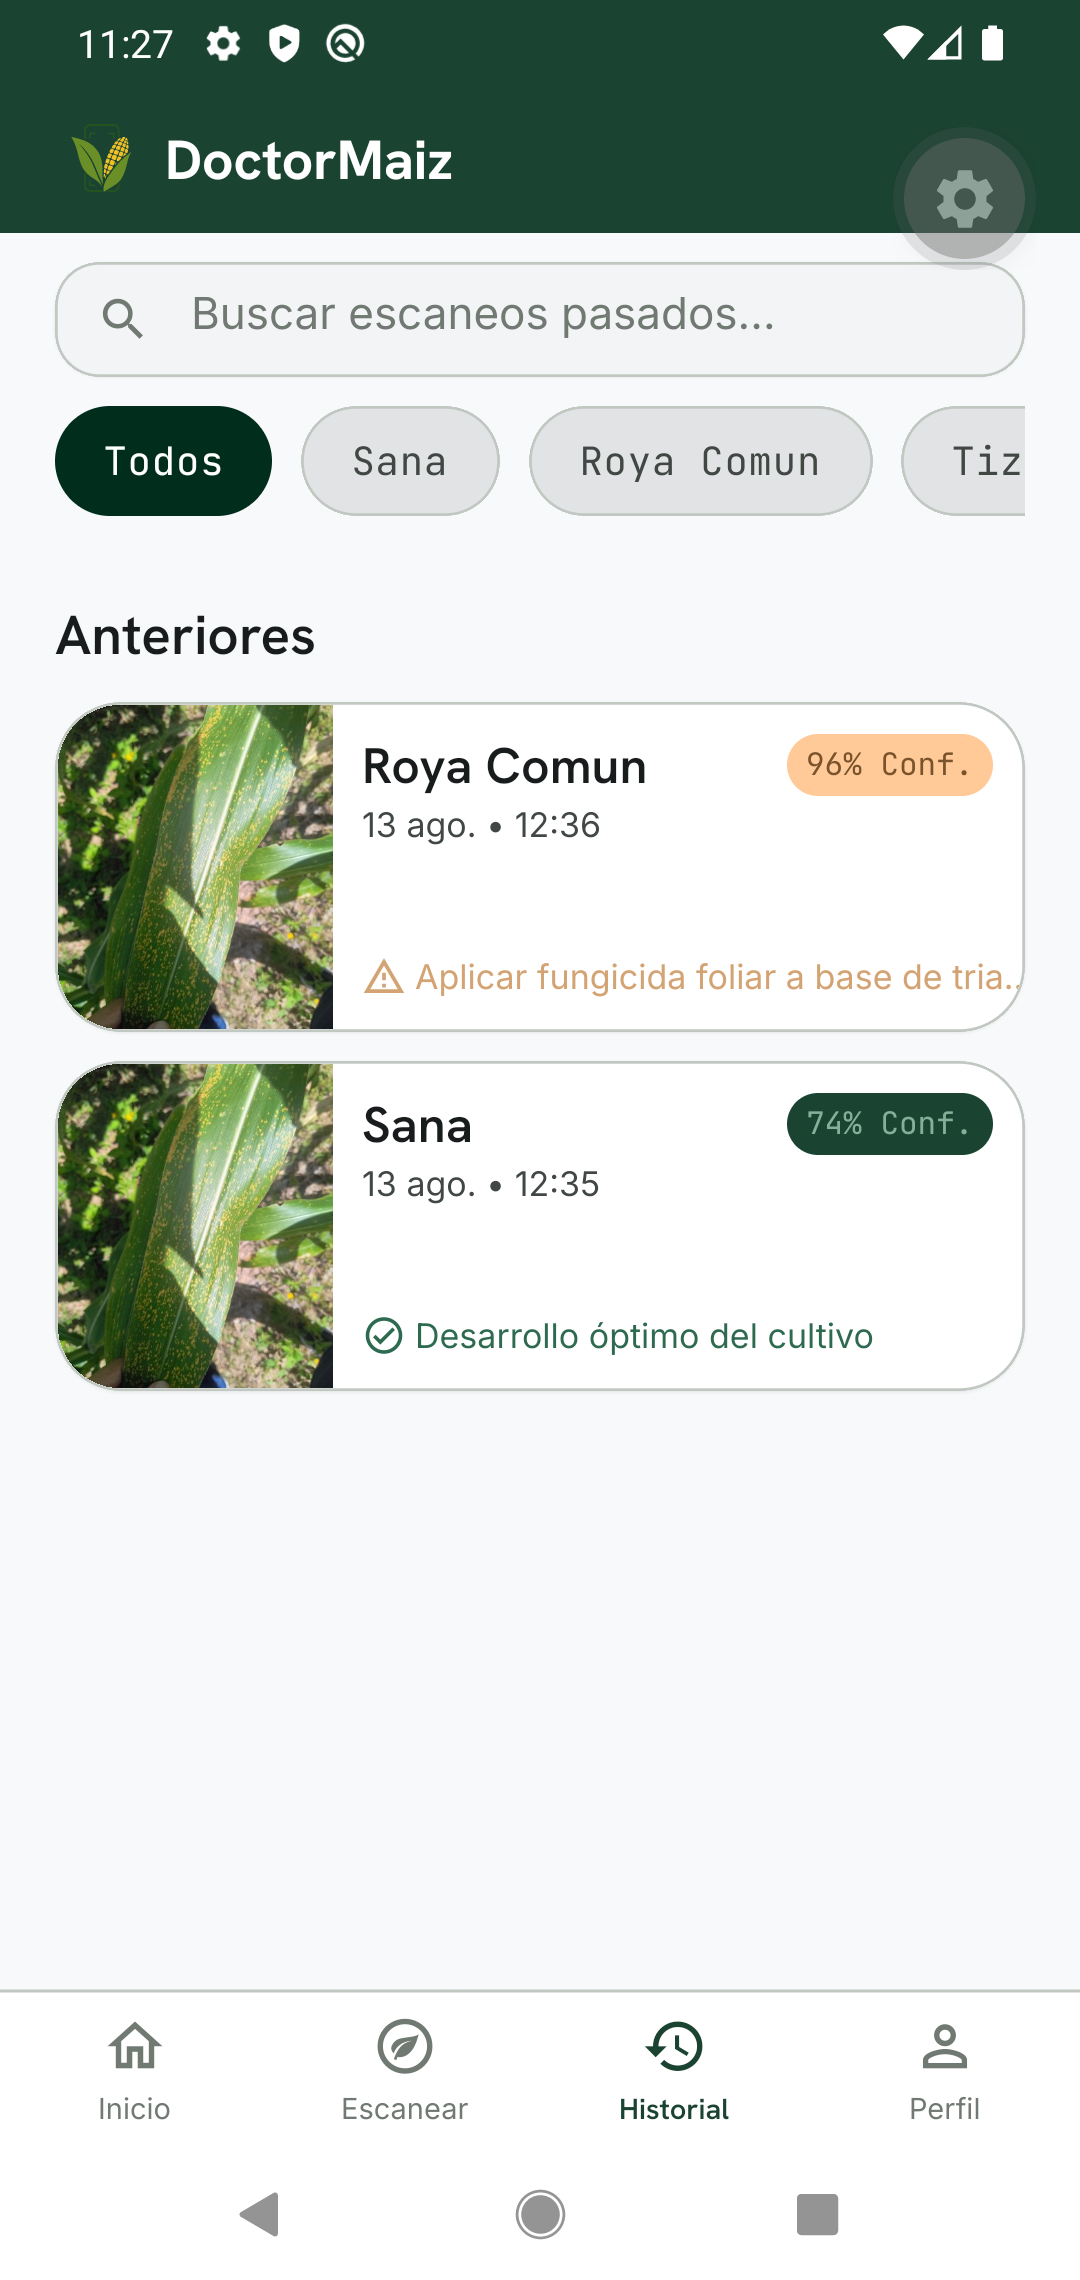
\includegraphics[width=0.46\linewidth]{img/pixel4_history.png}
    \caption{Pantalla de Historial: lista cronológica, buscador por texto y filtros rápidos por patología.}
    \label{fig:history_view}
\end{figure}

\section{Búsqueda y Filtros Rápidos}
En la parte superior de la pantalla cuentas con:
\begin{itemize}
    \item \textbf{Barra de búsqueda:} Escribe una palabra como «Roya» o una fecha para encontrar un registro específico.
    \item \textbf{Botones de filtro:} Toca \textbf{Todos}, \textbf{Sana}, \textbf{Roya Común} o \textbf{Tizón} para ver únicamente ese tipo de plantas en la lista.
\end{itemize}

\section{Cómo Hacer Seguimiento a un Tratamiento}
Cuando apliques un bioinsumo (por ejemplo, caldo de ceniza, *Trichoderma* o *Bacillus*), puedes usar el historial para comprobar si funcionó:
\begin{enumerate}
    \item Revisa en el historial la fecha y la ubicación de las plantas enfermas que escaneaste antes de la aplicación.
    \item Regresa al mismo sector del lote **7 a 10 días después**.
    \item Escanea las hojas nuevas que hayan crecido desde entonces.
    \item Si las hojas nuevas salen clasificadas como \textbf{Sana} o con nivel \textbf{Leve}, tu tratamiento frenó con éxito el avance del patógeno.
\end{enumerate}

% -------------------------------------------------------------
% CAPÍTULO 10: APORTE A LA CIENCIA (DATASET NACIONAL)
% -------------------------------------------------------------
\chapter{Aporte a la Ciencia: Dataset Nacional de Maíz}

En la pantalla de Inicio encontrarás el recuadro **«¡Sé parte de la Ciencia!»**. Esta herramienta permite que los agricultores compartan fotos de sus cultivos para entrenar y mejorar continuamente la inteligencia artificial.

\begin{figure}[H]
    \centering
    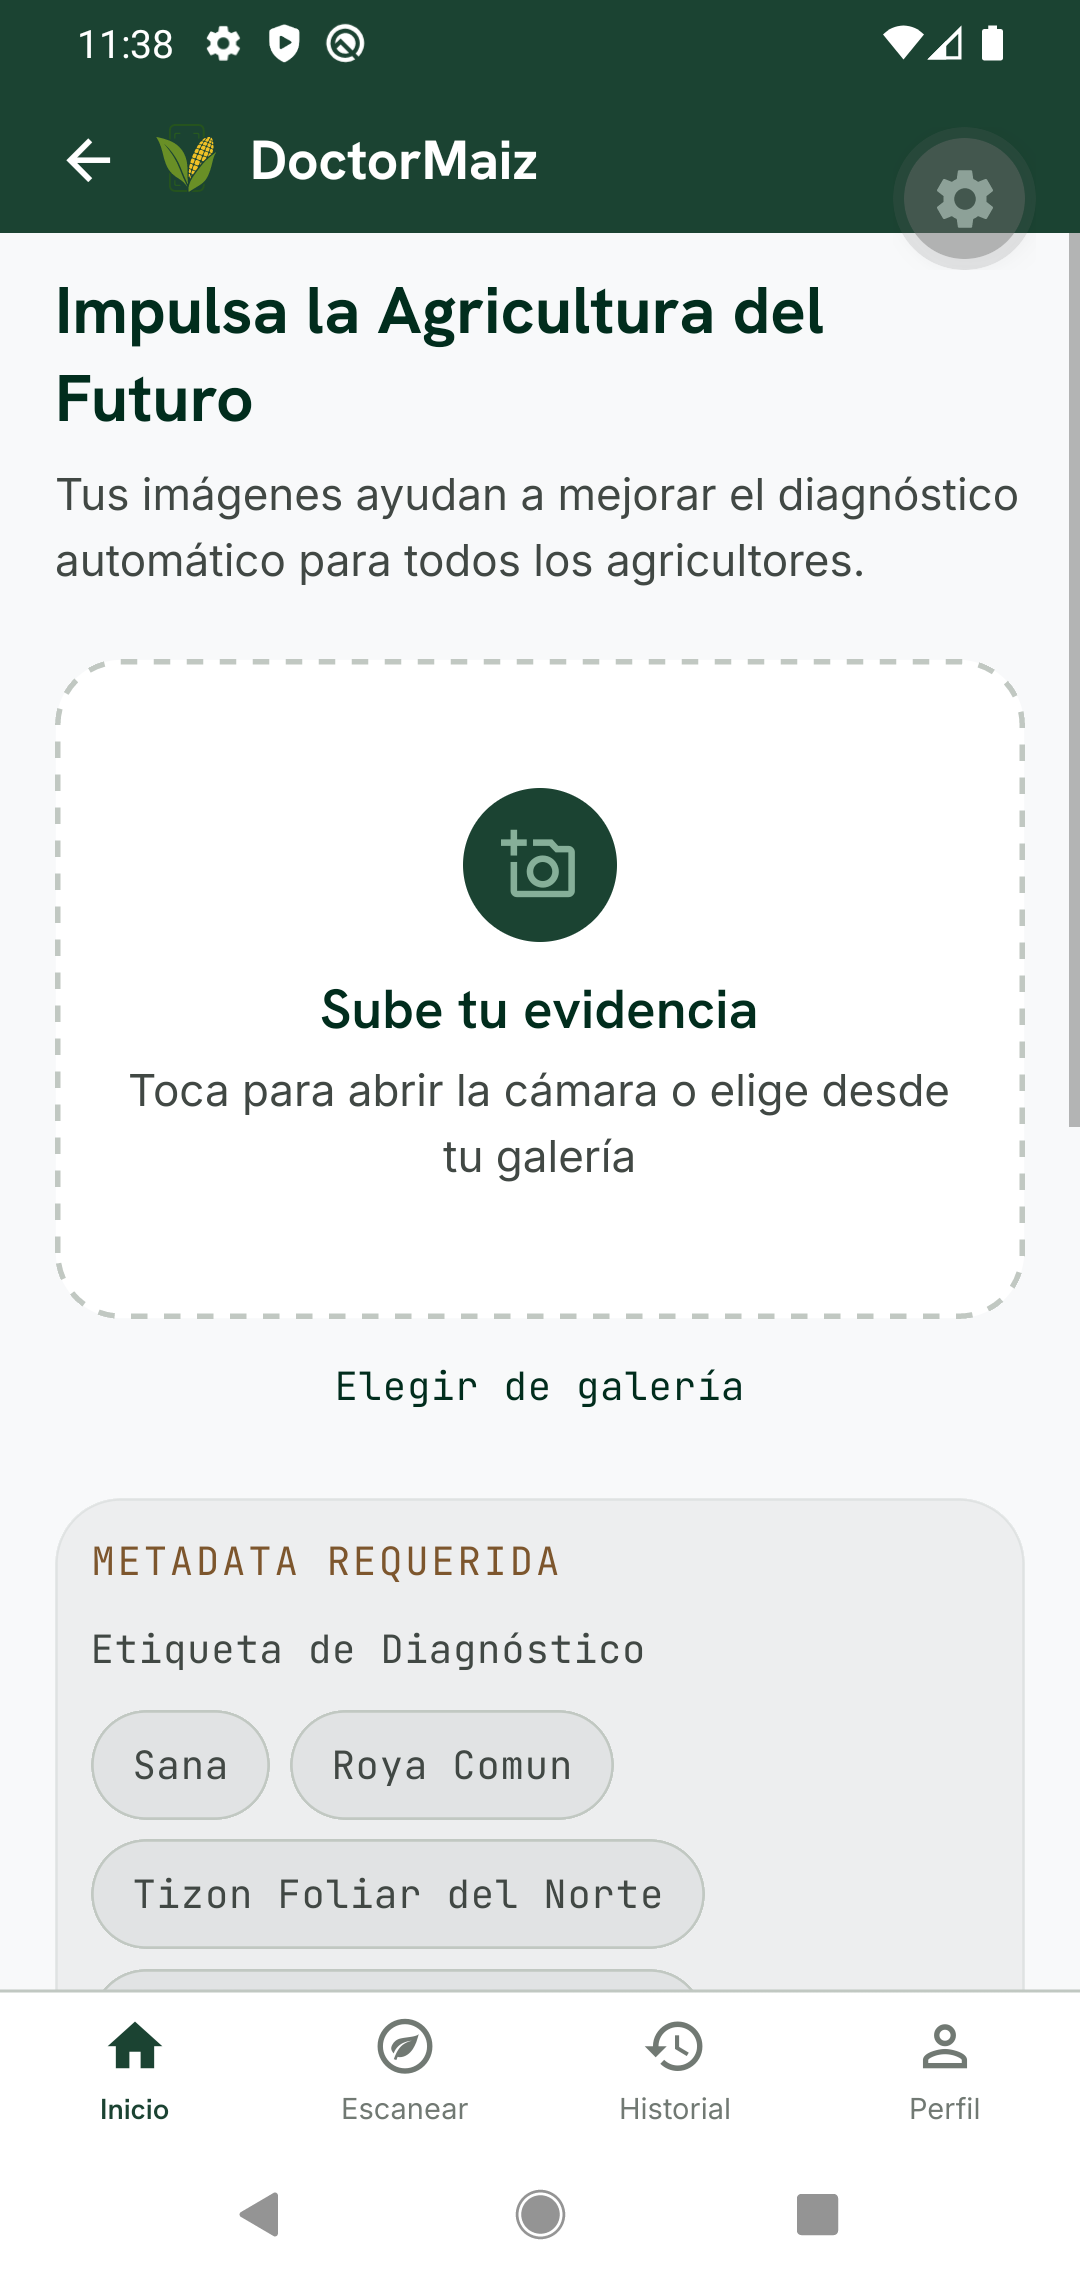
\includegraphics[width=0.46\linewidth]{img/pixel4_contribute.png}
    \caption{Pantalla de Contribución: sube fotos desde el campo para fortalecer el catálogo nacional.}
    \label{fig:contribute_view}
\end{figure}

\section{Cómo Subir tus Fotografías}
\begin{enumerate}
    \item Presiona el botón verde de la cámara en el centro del recuadro punteado, o bien toca **Elegir de galería**.
    \item En la sección **Metadata Requerida**, selecciona la etiqueta que mejor describa lo que viste en la planta (por ejemplo: *Sana*, *Roya Común*, *Tizón Foliar del Norte*).
    \item Si estás seguro del diagnóstico, confirma el envío.
    \item La fotografía se guardará en tu teléfono y se enviará al banco de datos colaborativo la próxima vez que te conectes a internet.
\end{enumerate}

% -------------------------------------------------------------
% CAPÍTULO 11: PREGUNTAS FRECUENTES Y SOLUCIÓN DE PROBLEMAS
% -------------------------------------------------------------
\chapter{Preguntas Frecuentes y Solución de Problemas}

\begin{description}
    \item[\textbf{¿Puedo usar la aplicación sin saldo de datos en el celular?}]
    Totalmente sí. Doctor Maíz tiene el modelo neuronal incorporado dentro de su propia instalación. Puedes poner el teléfono en modo avión o apagar los datos móviles y el escáner seguirá diagnosticando con la misma velocidad y precisión.

    \item[\textbf{¿Por qué el escáner me dice "No Reconocido"?}]
    Esto sucede si la foto quedó muy oscura, si la hoja se movió por una ráfaga de viento al disparar, o si la cámara enfocó el suelo o una planta que no es maíz. Vuelve a tomar la foto asegurándote de que la hoja de maíz llene la silueta punteada.

    \item[\textbf{El mapa no me muestra las fotos satelitales en el campo. ¿Qué hago?}]
    Las fotografías satelitales de alta resolución necesitan descargarse una vez desde internet. Antes de salir al lote, cuando estés en casa o en la cooperativa con Wi-Fi, abre la app y acércate en el mapa al lugar de tu parcela. Las imágenes quedarán guardadas en la memoria caché del teléfono y podrás verlas en el campo sin conexión.

    \item[\textbf{¿Se borran mis escaneos si se me apaga la batería?}]
    No. Cada escaneo se almacena inmediatamente en la memoria interna permanente del teléfono. Aunque el teléfono se apague por completo, al volverlo a encender todo tu historial y tus pines seguirán exactamente donde los dejaste.
\end{description}

% -------------------------------------------------------------
% APÉNDICE: ESCALAS CIENTÍFICAS HOMOLOGADAS
% -------------------------------------------------------------
\appendix
\chapter{Escalas Científicas Homologadas}

Para que las recomendaciones tengan respaldo agronómico formal, la Guía de Severidad de Doctor Maíz traduce a lenguaje llano las siguientes escalas científicas internacionales:

\begin{enumerate}
    \item \textbf{Roya Común (\textit{Puccinia sorghi}):} Escala diagramática Cobb modificada (\textit{Peterson et al., 1948}), con umbrales de severidad del 1\% al 5\% de área foliar afectada.
    \item \textbf{Tizón Foliar del Norte (\textit{Exserohilum turcicum}):} Escala de evaluación visual de \textit{Vieira et al. (2014)}, midiendo necrosis y coalescencia de lesiones elípticas.
    \item \textbf{Mancha Gris por Cercospora (\textit{Cercospora zeae-maydis}):} Escala estandarizada de \textit{Brito et al. (2007)}, basada en el avance rectangular entre nervaduras.
    \item \textbf{Complejo de Necrosis Letal del Maíz (MLN):} Escala visual de 5 grados estandarizada por el \textit{CIMMYT (Centro Internacional de Mejoramiento de Maíz y Trigo)}.
    \item \textbf{Gusano Cogollero (\textit{Spodoptera frugiperda}):} Escala de daño foliar de 1 a 9 grados de \textit{Davis, Ng \& Williams (1992)}, comúnmente utilizada en programas de mejoramiento y manejo integrado.
\end{enumerate}

\end{document}
